\documentclass{sig-alternate}
%\documentclass[conference]{IEEEtran}
%\documentclass[conference,final]{IEEEtran}

%\usepackage[numbers, sort, compress]{natbib}
\usepackage{graphicx}
\usepackage{amsmath}
\usepackage{amssymb}
\usepackage{color}
\usepackage{ifpdf}
%\usepackage{mdwlist}

%\usepackage{dcolumn}
\usepackage{float}
\usepackage[utf8]{inputenc}
\usepackage{multirow}
\usepackage{rotating}
\usepackage{subfigure}



%\usepackage[numbers, sort, compress]{natbib}
%\usepackage{latex8}
%\usepackage{float}
%\usepackage{times}    
\usepackage{url}
\usepackage{booktabs}
\usepackage{listings}   
\usepackage{paralist}    
\usepackage{wrapfig}    
%\usepackage[footnotesize,it]{caption}
\usepackage{multirow}
\usepackage{ifpdf}
%\usepackage{srcltx}
%\usepackage{subfigure}
\usepackage{xspace}
\usepackage{keyval}  
\usepackage{color}
\usepackage{comment}

\definecolor{listinggray}{gray}{0.95}
\definecolor{darkgray}{gray}{0.7}
\definecolor{commentgreen}{rgb}{0, 0.4, 0}
\definecolor{darkblue}{rgb}{0, 0, 0.4}
\definecolor{middleblue}{rgb}{0, 0, 0.7}
\definecolor{darkred}{rgb}{0.4, 0, 0}
\definecolor{brown}{rgb}{0.5, 0.5, 0}

\usepackage[normalem]{ulem}
\makeatletter
\def\cyanuwave{\bgroup \markoverwith{\lower3.5\p@\hbox{\sixly \textcolor{cyan}{\char58}}}\ULon}
\def\reduwave{\bgroup \markoverwith{\lower3.5\p@\hbox{\sixly \textcolor{red}{\char58}}}\ULon}
\def\blueuwave{\bgroup \markoverwith{\lower3.5\p@\hbox{\sixly \textcolor{blue}{\char58}}}\ULon}
\font\sixly=lasy6 % does not re-load if already loaded, so no memory problem.
\makeatother

\newif\ifdraft
\drafttrue
\ifdraft
\usepackage{xcolor}
\newcommand{\onote}[1]{ {\textcolor{cyan} { (***Ole: #1) }}}
\newcommand{\terminology}[1]{ {\textcolor{red} {(Terminology used: \textbf{#1}) }}}
\newcommand{\owave}[1]{ {\cyanuwave{#1}}}
\newcommand{\jwave}[1]{ {\reduwave{#1}}}
\newcommand{\alwave}[1]{ {\blueuwave{#1}}}
\newcommand{\jhanote}[1]{ {\textcolor{red} { ***shantenu: #1 }}}
\newcommand{\alnote}[1]{ {\textcolor{green} { ***andreL: #1 }}}
\newcommand{\amnote}[1]{ {\textcolor{blue} { ***andreM: #1 }}}
\newcommand{\smnote}[1]{ {\textcolor{brown} { ***sharath: #1 }}}
\newcommand{\pmnote}[1]{ {\textcolor{brown} { ***Pradeep: #1 }}}
\newcommand{\msnote}[1]{ {\textcolor{cyan} { ***mark: #1 }}}
\newcommand{\mrnote}[1]{ {\textcolor{purple} { ***melissa: #1 }}}
\definecolor{orange}{rgb}{1,.5,0}
\newcommand{\aznote}[1]{ {\textcolor{orange} { ***ashley: #1 }}}
\definecolor{dandelion}{cmyk}{0,0.29,0.84,0}
\newcommand{\mtnote}[1]{ {\textcolor{dandelion} { ***matteo: #1 }}}
\newcommand{\note}[1]{ {\textcolor{magenta} { ***Note: #1 }}}
\else
\newcommand{\onote}[1]{}
\newcommand{\terminology}[1]{}
\newcommand{\owave}[1]{#1}
\newcommand{\jwave}[1]{#1}
\newcommand{\alnote}[1]{}
\newcommand{\amnote}[1]{}
\newcommand{\aznote}[1]{}
\newcommand{\athotanote}[1]{}
\newcommand{\smnote}[1]{}
\newcommand{\pmnote}[1]{}
\newcommand{\jhanote}[1]{}
\newcommand{\msnote}[1]{}
\newcommand{\mtnote}[1]{}
\newcommand{\note}[1]{}
\newcommand{\mrnote}[1]{}
\fi

\newcommand{\cloud}{cloud\xspace}
\newcommand{\clouds}{clouds\xspace}
\newcommand{\pilot}{Pilot\xspace}
\newcommand{\pilots}{Pilots\xspace}
\newcommand{\pilotjob}{Pilot-Job\xspace}
\newcommand{\pilotjobs}{Pilot-Jobs\xspace}
\newcommand{\pilotcompute}{Pilot-Compute\xspace}
\newcommand{\pilotcomputes}{Pilot-Computes\xspace}
\newcommand{\pilotdata}{Pilot-Data\xspace}
\newcommand{\pilotdataservice}{Pilot-Data Service\xspace}
\newcommand{\pilotcomputeservice}{Pilot-Compute Service\xspace}
\newcommand{\computedataservice}{Compute-Data Service\xspace}
\newcommand{\pilotmapreduce}{PilotMapReduce\xspace}
\newcommand{\mrmg}{MR-Manager\xspace}
\newcommand{\pstar}{P*\xspace}
\newcommand{\pd}{PD\xspace}
\newcommand{\pj}{PJ\xspace}
\newcommand{\pjs}{PJs\xspace}
\newcommand{\pds}{Pilot Data Service\xspace}
\newcommand{\computeunit}{Compute-Unit\xspace}
\newcommand{\computeunits}{Compute-Units\xspace}
\newcommand{\dataunit}{Data-Unit\xspace}
\newcommand{\dataunits}{Data-Units\xspace}
\newcommand{\du}{DU\xspace}
\newcommand{\dus}{DUs\xspace}
\newcommand{\cu}{CU\xspace}
\newcommand{\cus}{CUs\xspace}
\newcommand{\su}{SU\xspace}
\newcommand{\sus}{SUs\xspace}
\newcommand{\schedulableunit}{Schedulable Unit\xspace}
\newcommand{\schedulableunits}{Schedulable Units\xspace}
\newcommand{\cc}{c\&c\xspace}
\newcommand{\CC}{C\&C\xspace}
\newcommand{\up}{\vspace*{-1em}}
\newcommand{\upp}{\vspace*{-0.5em}}
\newcommand{\numrep}{8 }
\newcommand{\samplenum}{4 }
\newcommand{\tmax}{$T_{max}$ }
\newcommand{\tc}{$T_{C}$ }
\newcommand{\tcnsp}{$T_{C}$}
\newcommand{\bj}{BigJob\xspace}
\newcommand{\MW}{Master-Worker\xspace}
\newcommand{\panda}{PanDA\xspace}
\newcommand{\apples}{AppLeS\xspace}

\newcommand{\I}[1]{\textit{#1}\xspace}
\newcommand{\B}[1]{\textbf{#1}\xspace}
\newcommand{\T}[1]{\texttt{#1}\xspace}
\newcommand{\C}[1]{\textsc{#1}\xspace}

\lstdefinestyle{myListing}{
  frame=single,   
  backgroundcolor=\color{listinggray},  
  %float=t,
  language=C,       
  basicstyle=\ttfamily \footnotesize,
  breakautoindent=true,
  breaklines=true
  tabsize=2,
  captionpos=b,  
  aboveskip=0em,
  belowskip=-2em,
  %numbers=left, 
  %numberstyle=\tiny
}      

\lstdefinestyle{myPythonListing}{
  frame=single,   
  backgroundcolor=\color{listinggray},  
  %float=t,
  language=Python,       
  basicstyle=\ttfamily \footnotesize,
  breakautoindent=true,
  breaklines=true
  tabsize=2,
  captionpos=b,  
  %numbers=left, 
  %numberstyle=\tiny
}



%  \setlength{\parskip}{0.05ex} % 1ex plus 0.5ex minus 0.2ex}
%  \setlength{\parsep}{0pt}
%  %\setlength{\headsep}{0pt}
%  \setlength{\topskip}{0pt}
%  \setlength{\topmargin}{0pt}
%  %\setlength{\topsep}{0pt}
%  \setlength{\partopsep}{0pt}

% This is now the recommended way for checking for PDFLaTeX:


\ifpdf
\DeclareGraphicsExtensions{.pdf, .jpg, .tif}
\else
\DeclareGraphicsExtensions{.eps, .jpg, .ps}
\fi

\tolerance=1000
\hyphenpenalty=10

\usepackage{lscape}

\usepackage{listings}

\lstnewenvironment{code}[1][]%
{
\noindent
%\minipage{0.98 \linewidth} 
\minipage{1.0 \linewidth} 
\vspace{0.5\baselineskip}
\lstset{
    language=Python,
%    numbers=left,
%    numbersep=4pt,
    frame=single,
    captionpos=b,
    stringstyle=\ttfamily,
    basicstyle=\scriptsize\ttfamily,
    showstringspaces=false,#1}
}
{\endminipage}

\begin{document}
\conferenceinfo{HPDC'13}{2013, New York, USA}
% \conferenceinfo{ECMLS'11,} {June 8, 2011, San Jose, California, USA.}
% \CopyrightYear{2011}
% \crdata{978-1-4503-0702-4/11/06}
% \clubpenalty=10000
% \widowpenalty = 10000

\title{A Fresh Perspective on Pilot-Jobs}

% \alignauthor
% Ben Trovato\titlenote{Dr.~Trovato insisted his name be first.}\\
%        \affaddr{Institute for Clarity in Documentation}\\
%        \affaddr{1932 Wallamaloo Lane}\\
%        \affaddr{Wallamaloo, New Zealand}\\
%        \email{trovato@corporation.com}
% % 2nd. author
% \alignauthor
% G.K.M. Tobin\titlenote{The secretary disavows
% any knowledge of this author's actions.}\\
%        \affaddr{Institute for Clarity in Documentation}\\
%        \affaddr{P.O. Box 1212}\\
%        \affaddr{Dublin, Ohio 43017-6221}\\
%        \email{webmaster@marysville-ohio.com}
% % 3rd. author
% \alignauthor Lars Th{\o}rv{\"a}ld\titlenote{This author is the
% one who did all the really hard work.}\\
%        \affaddr{The Th{\o}rv{\"a}ld Group}\\
%        \affaddr{1 Th{\o}rv{\"a}ld Circle}\\
%        \affaddr{Hekla, Iceland}\\
%        \email{larst@affiliation.org}
% \and  % use '\and' if you need 'another row' of author names
% % 4th. author
% \alignauthor Lawrence P. Leipuner\\
%        \affaddr{Brookhaven Laboratories}\\
%        \affaddr{Brookhaven National Lab}\\
%        \affaddr{P.O. Box 5000}\\
%        \email{lleipuner@researchlabs.org}
% % 5th. author
% \alignauthor Sean Fogarty\\
%        \affaddr{NASA Ames Research Center}\\
%        \affaddr{Moffett Field}\\
%        \affaddr{California 94035}\\
%        \email{fogartys@amesres.org}
% % 6th. author
% \alignauthor Charles Palmer\\
%        \affaddr{Palmer Research Laboratories}\\
%        \affaddr{8600 Datapoint Drive}\\
%        \affaddr{San Antonio, Texas 78229}\\
%        \email{cpalmer@prl.com}
% }

\date{}
\maketitle

\begin{abstract} 
  There is no agreed upon definition of \pilotjobs; however a
  functional attribute of \pilotjobs that is generally agreed upon is
  they are tools/services that support multi-level and/or
  application-level scheduling by providing a scheduling overlay on
  top of the system-provided schedulers.  \aznote{Not sure it is good
    to open our abstract stating the confusion/uncertainty inherent
    in defining Pilot-Jobs...  perhaps first state our motivation for
    this work (``aim(ing) to provide appropriate context, insight, and
    analysis of a \pilotjobs, and thereby bring about a hitherto
    missing consilience...'')  and then state that it's somewhat
    controversial?  I see where it could be eye-catching to outright
    state that there IS controversy/uncertainty though, and that we
    are aiming to quash it.  Making this note to try and figure this
    out :)} Nearly everything else is either specific to an
  implementation, open to interpretation or not agreed upon. For
  example, are \pilotjobs part of the application space, or part of
  the services provided by an infrastructure? We will see that
  close-formed answers to questions such as whether \pilotjobs are
  system-level or application-level capabilities are likely to be
  elusive. Hence, this paper does not make an attempt to provide
  close-formed answers, but aims to provide appropriate context,
  insight and analysis of a large number of \pilotjobs, and thereby
  bring about a hitherto missing consilience in the community's
  appreciation of \pilotjobs.  Specifically this paper aims to provide
  a comprehensive survey of \pilotjobs, or more generically of
  \pilotjob like capabilities.  \aznote{Is a ``comprehensive survey''
    still true given last week's discussion of focusing on
    ``landmark'' pilotjobs?}  A primary motivation for this work stems
  from our experience when looking for an interoperable, extensible
  and general-purpose \pilotjobs; in the process, we realized that
  such a capability did not exist. The situation was however even more
  unsatisfactory: in fact there was no agreed upon definition or
  conceptual framework of \pilotjobs.  To substantiate these points of
  view, we begin by sampling (as opposed to a comprehensive survey)
  ~\onote{a few lines above we say that we're doing a comprehensive
    survey!} some existing \pilotjobs and the different aspects of
  these \pilotjobs, such as the applications scenarios that they have
  been used and how they have been used. The limited but sufficient
  sampling highlights the variation, and also provides both a
  motivation and the basis for developing an implementation agnostic
  terminology and vocabulary to understand \pilotjobs; Section \S3
  attempts to survey the landscape/eco-system of \pilotjobs.  With an
  agreed common framework/vocabulary to discuss and describe
  \pilotjobs, we proceed to analyze the most commonly utilized
  \pilotjobs and in the process provide a comprehensive survey of
  \pilotjobs, insight into their implementations, the infrastructure
  that they work on, the applications and application execution modes
  they support, and a frank assessment of their strengths and
  limitations.  An inconvenient but important question -- both
  technically and from a sustainability perspective that must be
  asked: why are there so many similar seeming, but partial and
  slightly differing implementations of \pilotjobs, yet with very
  limited interoperability amongst them?  Examining the reasons for
  this state-of-affairs provides a simple yet illustrative case-study
  to understand the state of the art and science of tools, services
  and middleware development.  Beyond the motivation to understand the
  current landscape of \pilotjobs from both a technical and a
  historical perspective, we believe a survey of \pilotjobs is a
  useful and timely undertaking as it provides interesting insight
  into understanding issues of software sustainability.
  % believe that a survey of \pilotjobs provides and appreciation for
  % the richness of the \pilotjobs landscape.  is
  % not to discuss the \pstar conceptual framework, but That led to
  % the \pstar model.
\end{abstract}

\section{Introduction} 

\jhanote{Please use macros! e.g., for consistency between PJ sytems
  and \pilot systems and \pilotjob systems. similarly for M-W}

\jhanote{Generally not good style to begin new subsection immediately
  after section starting}

The seamless uptake of distributed infrastructures by scientific
applications has been limited by the lack of pervasive and
simple-to-use abstractions at multiple levels – at the development,
deployment and execution stages. Of all the abstractions proposed to
support effective distributed resource utilization, a survey of actual
usage suggested that \pilotjobs were arguably one of the most
widely-used distributed computing abstractions – as measured by the
number and types of applications that use them, as well as the number
of production distributed cyberinfrastructures that support them.

\jhanote{Now develop the following paragraph along the lines of: Why
  have \pilotjobs been successful?}

The fundamental reason for the success of the \pilotjob abstraction is that
\pilotjobs liberate applications/users from the challenging requirement of
mapping specific tasks onto explicit heterogeneous and dynamic resource pools.
In other words, at least in part, due to the decoupling between task/workload
specification and task management. \pilotjobs also improve the efficiency of
task assignment and shield applications from having to load-balance tasks
across such resources.\onote{not sure if 'load-balance'  is appropriate here} 
Another concern often addressed by \pilotjobs is fault
tolerance which commonly refers the ability of the \pilotjob system to verify
the execution environment before executing jobs. The \pilotjob abstraction is
also a promising route to address specific requirements of distributed
scientific applications, such as coupled-execution and application-level
scheduling~\cite{ko-efficient,DBLP:conf/hpdc/KimHMAJ10}.

%   \onote{I think the most important reasons why Pilot Jobs being so
%     popular (and re-invented over and over again) is that they allow
%     the execution of small (i.e., singe / few-core) tasks efficiently
%     on HPC infrastrucutre by massively reducing queueing time. HPC
%     sites (from schedulers to policies) have always been (and still
%     are) discrimatory against this type of workload in favor of the
%     large, tightly-coupled ones. Pilot-Jobs try to counteract. While
%     this is certainly not the main story that we want to tell, this
%     should IMHO still be mentioned. } \jhanote{This is definitely one
%     of the main reasons, but as Melissa pointed out it during RADICAL
%     call, it is by no means the only reason. Need to get the different
%     reasons down here.. then find a nice balance and description}

\jhanote{Although pilotjobs have solved/addressed many problems, now
    develop the problem with \pilotjobs themselves..}
A variety of PJ frameworks have emerged: Condor-G/
Glide-in~\cite{condor-g}, Swift~\cite{Wilde2011},
DIANE~\cite{Moscicki:908910}, DIRAC~\cite{1742-6596-219-6-062049},
PanDA~\cite{1742-6596-219-6-062041}, ToPoS~\cite{topos},
Nimrod/G~\cite{10.1109/HPC.2000.846563}, Falkon~\cite{1362680} and
MyCluster~\cite{1652061} to name a few. Although they are all, for the
most parts, functionally equivalent -- they support the decoupling of
workload submission from resource assignment -- it is often impossible
to use them interoperably or even just to compare them functionally or
qualitatively.  The situation is reminiscent of the proliferation of
functionally similar yet incompatible workflow systems, where in spite
of significant a posteriori effort on workflow system extensibility
and interoperability (thus providing post-facto justification of its
needs), these objectives remains difficult if not infeasible.

\section{A Preliminary Survey of Existing Pilot-Jobs Systems}
\label{sec:survey}

%\subsection{A Functional Approach to Pilot-Jobs}
%Many scientific communities began running into the same issues: 

As distributed systems grew in capacity and capability, they also grew
in complexity and heterogeneity. For example, many machines
implemented their own batch queuing systems, and oftentimes these
systems varied from machine to machine.  The wide use of heterogenous
resources, resulted in the need for workload management across these
resources.  In order to harness the power of these heterogeneous
resources to run jobs, one particular solution proposed is that of
\pilotjobs

% , which have historically been used as a means of solving these
% issues.
% This gave rise to the the need for job submission management via batch
% queuing systems and middleware access also grew.
%We briefly discuss some specific uses of \pilotjobs below.

\pilotjobs are most commonly used for the execution of many tasks
through the use of a container job. They are often measured by
their throughput, that is, the number of tasks that they can complete
per second (tps), or alternatively, by the total number of tasks
executed. As such, \pilotjobs are used to achieve
high-throughput, for example, when using genome sequencing techniques
or ensemble-based applications. \pilotjobs have also been used for
parameter sweeps, chained tasks, and loosely-coupled but distinct
tasks. %note to self: cite these with papers

Multi-scale simulations have also benefited from the use of
\pilotjobs. A framework for load balancing via dynamic resource
allocation for coupled multi-physics (MPI-based) simulations using
\pilotjobs was demonstrated in Ref.~\cite{ko-efficient}.
This was achieved by dynamically assigning more processors to
jobs with longer runtimes, so that these jobs could accomplish their workload
in the same amount of wall-clock time as those with shorter runtimes.
This led to an overall reduction of jobs that were waiting to communicate
via MPI, and an overall reduction of the total simulation runtime. 

\pilotjobs can be used for  simulations
 with varying numbers of tasks to complete, for example,
molecular dynamics simulations requiring task restart. These types of 
 simulations may start with a fixed number of tasks but spawn 
 more tasks in order to continue simulating. \pilotjobs can be
utilized for these types of dynamic simulations, because 
new tasks can be fed to the \pilot at any time within a given 
runtime. Without \pilotjobs, these simulations would have to 
be resubmitted to the batch queue and wait for their time
to become active again~\cite{luckow2009adaptive}.

\pilotjobs have also been used to avoid queue wait times for many jobs
as well as harness and utilize different resources (with different
batch queueing systems) to do \textit{scale-across} simulations.
As a fault tolerant mechanism, many \pilotjob systems monitor
failed jobs and have the ability to restart them within the given 
time frame of the \pilotjob's total runtime~\cite{1742-6596-219-6-062049,condor-g,nilsson2011atlas}. 

\subsection{Historical Context}

In order to appreciate \pilotjobs, we outline the evolution of
\pilot-like capabilities ultimately leading to the creation of the
first actual \pilotjob. We present a brief chronological order of
\pilotjob-like systems, beginning with simple Master-Worker-based
applications through advanced workload management systems.

\subsubsection*{The Evolution of \pilotjobs} 

Interestingly we find that \pilotjobs have been used even before they
were named as such; we refer to these as pre-\pilotjob systems, a
prominent example of which is the Master-Worker (M-W) scheme and
associated frameworks.  In the context of distributed systems, the M-W
scheme was initially used of farming tasks from a master to a various
number of workers, and could easily be adapted to run in a
platform-independent way across the potentially heterogeneous
resources~\cite{masterworker, Goux00anenabling}. Master-Worker based
frameworks could respond to the dynamically changing resources by
adapting the number of workers to match the resource availability.

%Although Master-Worker schemes were important, they
%required application modification. \jhanote{last statement is unclear}
%\onote{I don't think that I agree with this 
%statement. There are lots of independent master-worker frameworks, libraries 
%and tools out there. What does 'application modification' mean here?}

BOINC is a volunteer-based, distributed master-worker framework that
also pre-dated \pilotjob
systems~\cite{Anderson:2004:BSP:1032646.1033223}. BOINC plays a
significant role in distributed computing in that it utilizes unused
computer cycles on the client-side in order to execute tasks given
from the server-side. Applications can be built on top of BOINC for
their own scientific endeavors; it was originally built for the
SETI@Home project, which uses Internet-connected computers to download
and analyze radio telescope data. Most often, these computers are
based around the world -- users merely have to download the client
program, and it runs in the background on their computer. The data is
then aggregated back on the server-side and analyzed. The idea of
farming out tasks in a distributed environment including personal
computers was powerful in that it essentially made a grid out of many
less powerful machines.

As the resources in the grid adopted more and more batch queuing
systems, users were forced to submit their jobs individually to a
scheduler. Oftentimes, the type of scheduler on a certain machine was
different than that of another machine. There was a need for managing
the heterogenous, dynamic grid environments, especially in terms of
dynamic scheduling. This drove the creation of
AppLeS~\cite{Berman:2003:ACG:766629.766632}, a framework for
application-level scheduling. For this purpose, AppLeS provides an
agent that can be embedded into an application enabling the
application to acquire resources (e.\,g.\ via Globus, SSH or Legion)
and efficiently schedule tasks onto these. Further, AppLeS provides
different application templates, e.\,g.\ for parameter sweep,
master-worker and moldable parallel applications.

The rise of application-level scheduling, as in AppLeS, opened new
possibilities to Grid environments. The concept of application-level
scheduling was extended to include long-term performance prediction in
heterogenous Grid environments via the Grid Harvest Service (GHS)
system~\cite{ghs}. GHS provides a prediction model that was derived by
probability analysis and simulation and useful for large-scale
applications in shared environments. Its prediction models and task
scheduling algorithms are utilized in the placement of tasks across
Grid resources. GHS supports three classes of task scheduling: (i)
single task, (ii) parallel processing, and (iii) meta-task. The
performance evaluation and modeling in conjunction with task-specific
management (such as placement, scheduling, and execution) allows the
utilization of many heterogenous resources in an efficient manner.

Although pre-pilot systems, such as AppLeS, gave user-level control of
scheduling, queue reservation time still was an issue. This brought
about the idea of placeholder
scheduling~\cite{Pinchak02practicalheterogeneous,
  Singh:2008:WTC:1341811.1341822}. A placeholder was an early \pilot
mechanism in that it was an abstraction layer above the various batch
queuing systems available on different resources. It held a
\textit{place} in the regular batch queue, and when it became active,
it could pull tasks to execute.  Placeholder scheduling was
advantageous in that it did not require any special superuser
privileges on the machines, which was something most grid users did
not have access to. It also provided a means of load balancing across
the different resources. As placeholder scheduling evolved, it came to
include dynamic monitoring and throttling of the different
placeholders based on the queue times on the machines.

Placeholder scheduling, or early \pilots, evolved to encompass complex
workload management systems. Such complex systems will be discussed in
depth in Section \ref{sec:pj}. As applications began to utilize
distributed cyberinfrastructure, the workloads grew from small sets of
short running jobs to many jobs with either short or potentially long
runtimes. There was a need for more complex management of these
workloads and additional capabilities for user-level control of the
tasks that would be executed within the placeholder job. This drove
the creation of the modern idea of \pilots.
 
% Cite: Work Queue: http://www3.nd.edu/~ccl/research/papers/wq-python-pyhpc2011.pdf 
% Work queue is not based on pilots but is an interesting read for ensemble-based scientific applications on grids using python

\subsection{Informal Description of Pilot-Job Systems}
\label{sec:pj}

\note{talk about tool development, unregulated cottage industry - Why
  is that? diverse low-level infrastructure, no incentive to use
  multiple infrastructures? External vs.  internal perspective?}

As stated above, \pilotjobs provide the ability to distribute workload
across multiple systems and provide an easy way to schedule many jobs
at one time. This in turn improves the utilization of resources,
reduces the net wait time of a collection of tasks, and also prevents
saturation of resource batch queuing systems from high-throughput
simulations where many jobs need to be run at one time.

\subsubsection{Criteria and Classifications}

We survey the \pilotjob systems according to different 
functional and non-functional criteria. Further we analyze the internal 
architecture of each \pilotjob system.

\jhanote{I don't think we should say we ``assess'' according to these
  different criteria, but we should say that a brief survey of the
  \pilotjob literatures shows that many different and often
  inconsistent criteria have been used. then we need to add some
  criteria of our own stating that based upon our
  literature/understanding we think it will be useful to develop
  further criteria... Also, it is important to note that not all
  criteria are used for every \pilotjob system}


\emph{Functional Features:} The functional criteria describe the
capabilities of the \pilotjob system: (i) What use cases? What
applications types and usage modes are supported (MPI, ensembles,
workflows)?, (ii) What abstraction and user interface is provided to
the developer: API, CLI, web service, web portal?, (iii) Does the
\pilotjob system support distribution?, (iv) Are there any
higher-level tools available for \pilotjob system (e.g. workflow
systems, data analysis systems)?, (v) Does the \pilotjob system
support data?, (vi) What types of infrastructure are supported (HTC,
HPC, cloud)? Does the \pilotjob system provide interoperability
support? and (vii) does the framework support advanced workload
management capabilities (e.g. the automatic provisioning of \pilots).

\emph{Non-Functional Features:} Non-functional features describe the characteristics and behavior of a
\pilotjob system and are not directly related to a specific function or
capability of the \pilotjob system. Non-functional properties include: (i)
performance, (ii) scalability (task throughput, number resources/slots), (iii)
fault tolerance, (iv) interoperability and (v) security.

The performance and scalability define the response times and size of the
workload a user can expect to be supported. Security describes the security
mechanisms used by the framework, e.\,g.\ for authentication of the user, for
securing the communication protocol and for sandboxing the application.
Further, some \pilotjobs solely support single users, while more complex
\pilot-based workload managers commonly support multiple users (e.\,g.\ using
glexec).


\alnote{we might want to consider to merge internal and non-functional}
\emph{Internal Aspects:} Internal features of a \pilotjob system include: (i)
the architecture of the system (layers, sub-systems, communication \&
coordination, central vs. decentral architectures; push vs. pull model,
agent-based; number of supported resource types), (ii) resource access layer:
What low-level infrastructures/middleware are supported? How interoperable is
the framework (vertically, horizontally)?, (iii) the deployment model: hosted
service versus tool/library, application vs. system-level, (iv) how is the
workload managed and scheduled (supported algorithms, support for
application-level scheduling, data-compute scheduling, resource
acquisition/release policies, dispatch policies, number of scheduling levels)
and (v) does the framework have dependencies to other third-party
components/services?



\subsubsection{Pilot-Job Systems Overview}

\begin{figure}[t]
	\centering
		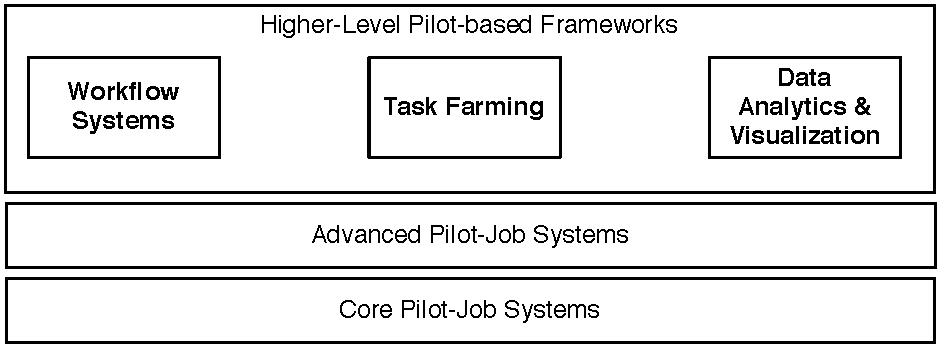
\includegraphics[width=0.45\textwidth]{figures/classification}
	\caption{Pilot-Job Classification: Different PJ systems focus
          on different parts of the distributed computing stack: (i)
          PJ systems that solely provide the \pilot capability, (ii)
          systems that offer resource management capabilities based on
          \pilots and (iii) applications, tools and services that
          utilize \pilots for resource management. \jhanote{we should
            change the ``higher-level pilot-based frameworks'' to
            ``higher-level frameworks that can use pilot-jobs''.}}
        \alnote{mention that these layers are not cleanly separated:
          Pegasus is constraint to a single PJ system (Corral)}
	\label{fig:figures_classification}
\end{figure}


As shown Figure~\ref{fig:figures_classification}, PJ systems operate
on different levels of the distributed computing stack: (i) Core PJ
systems that solely provide a simple \pilot capability, (ii) systems
that provide resource management capabilities based on \pilots and
(iii) applications, tools and services that utilize
\pilots. \jhanote{the mapping of the above to the different levels in
  the diagram is implied, but the text above does not guide/make it
  explicit. Please refine}

\subsubsection*{Core Pilot-Job Systems}

Core \pilotjob systems focus on the basic \pilot capabilities, i.\,e.\ the
provisioning of the placeholder job capability. Various Master-Worker systems
that provide such a mechanism (e.\,g.\
Nimrod-G~\cite{10.1109/HPC.2000.846563}). Condor-G/Glide-In is the most
well-known \pilotjob system. Further examples for lightweight \pilotjob
systems are: ToPos~\cite{topos},
MyCluster~\cite{Walker:2007:PAC:1285840.1285848},
GridBot~\cite{Silberstein:2009:GEB:1654059.1654071} and LGI~\cite{lgi}.

Nimrod-G~\cite{10.1109/HPC.2000.846563}, DIANE~\cite{diane-thesis} and Work
Queue~\cite{workqueue-pyhpc2011} are examples of Master-Worker systems that
utilize a placeholder agent that dispatches and manages tasks. For example,
Nimrod-G utilizes a Job Wrapper that is responsible for pulling a task and its
associated data and then manages the execution of this task. While modern
\pilotjobs often acquire resources opportunistically and then distribute tasks
to resources they were able to acquire, Nimrod-G utilizes a central,
cost-based scheduler.

Condor-G/Glide-in~\cite{condor-g} is one of the pioneers of the \pilotjob
concept. Glide-in is a mechanism by which user can add remote grid resources
to the local condor pool and run their jobs on the added resource the same way
that all condor jobs are submitted. A Glide-in is submitted using the Condor-G
grid universe. On the remote resource a set of Condor daemons (e.\,g.\ the
startd daemon) is started, which then registers the available job slots with
the central Condor pool. The resources added are available only for the user
who added the resource to the pool, thus giving complete control over the
resources for managing jobs without any queue waiting time. Glide-in installs
and executes necessary Condor daemons and configuration on the remote
resource, such that the resource reports to and joins the local Condor pool.
Glide-in is limited in that the daemons must be running on a given resource,
meaning that this process must be approved by resource owners or system
administrators. Various systems that built on the \pilot capabilities of 
Condor-G/Glide-in have been developed, e.\,g.\ Bosco~\cite{bosco} and 
GlideinWMS. Bosco e.\,g.\ simplifies the process of spawning a Glide-in 
significantly.



% Venus-C~\cite{venusc-generic-worker} provides a \pilotjob-like
% capability on Microsoft Azure clouds called a Generic Worker. The
% Generic Worker creates a layer of abstraction above the inner workings
% of the cloud.  The idea behind the Generic Worker is to allow
% scientists to do their science without requiring knowledge of backend
% HPC systems by offering e-Science as a service. Venus-C has not been
% shown to work with grids, because its main objective is to motivate
% scientists to use cloud infrastructures.  While the notion of moving
% to the cloud for data-driven science is an important one, many
% existing cyberinfrastructures still have powerful grid computers that
% can also be leveraged to assist with the data-driven computations.



%%%%%%%%%%%%%%%%%%%%
\subsubsection*{Advanced Pilot-Job Systems}
%  \pilot-based Workload Manager, Systems for Multi-Level Scheduling}


%AppLeS~\cite{Berman:2003:ACG:766629.766632} is a framework for 
%application-level scheduling. For this purpose, AppLeS provides an agent that 
%can be embedded into an application enabling the application to acquire 
%resources (e.\,g.\ via Globus, SSH or Legion) and efficiently schedule tasks 
%onto these. Further, AppLeS provides different application templates,
%e.\,g.\ for parameter sweep, master-worker and moldable parallel applications.

\jhanote{AppLeS is not strictly \pilotjob based?  but \pilotjob like
  capabilities?} \alnote{The question is: when is a \pilot a \pilot?
  When the use the term \pilot and when \pilot-like? Apples has a
  component -- the Actuator (Quote from paper: "... handles task
  launching, polling, and cancellation ..."), which is quite similar
  to a \pilot. But maybe AppLeS is something for the history section
  or a separate category for Master/Worker frameworks...  PJ evolved
  from the need to map master/worker style computations to
  heterogeneous, dynamic distributed grid environments. Added a
  pre-\pilot category to the history sub-section.}

While core PJ systems mainly focus on providing simple \pilot capabilities 
commonly in application space, many of these systems evolved towards more 
\pilot-based workload managers, which are often centrally hosted moving 
critical functionality from the client to the server. These systems usually 
deploy \pilot factories that automatically start new \pilots on demand and 
integrate security mechanisms to support multiple users. Several of these have 
been developed in the context of the LHC experiment at CERN, e.\,g.\ 
GlideInWMS, Dirac~\cite{1742-6596-219-6-062049}, 
PanDa~\cite{1742-6596-331-7-072069}, AliEn~\cite{1742-6596-119-6-062012} and 
Co-Pilot~\cite{copilot-tr}. Each of these \pilots serves a particular user 
community and experiment.

GlideinWMS~\cite{1742-6596-119-6-062044} is a higher-level workload management
system that is based on the \pilot capabilities of Condor-G/Glide-in. The
system can based on the current and expected number of jobs in the pool,
automatically increase or decrease the number of active Glide-ins (\pilots)
available to the pool. GlideinWMS is a multi-user \pilotjob system commonly
deployed as a hosted service. In contrast to low-level \pilotjob systems,
GlideinWMS attempts to hide rather than expose the \pilot capabilities from
the user. GlideinWMS is currently deployed in production on OSG and is the
recommended mode for accessing OSG resources.

The PanDA~\cite{1742-6596-331-7-072069} workload management systems is also 
based on Condor-G/Glidein. In contrast, a Condor-G only approach,
PanDA can utilize multiple queues; each \pilot is assigned to a certain PanDA
internal queue. PanDA also provides the ability to manage data associated the 
jobs managed by the PanDA workload manager.

AliEn~\cite{1742-6596-119-6-062012} also provides the ability to tightly 
integrate storage and compute resources and is also able to manage file 
replicas. While all data can be accessed from anywhere, the scheduler is aware 
of data localities and attempts to schedule compute close to the data.

Dirac~\cite{1742-6596-219-6-062049} is another comprehensive workload
management system built on top of \pilots. As PanDA and AliEn it supports the
management of data, which can be placed in different kinds of storage elements
(e.\,g.\ based on SRM).

Another interesting \pilot that is used in the LHC context is
Co-Pilot~\cite{copilot-tr}. Co-Pilot serves as integration point between
different grid \pilotjob systems (such as AliEn and PanDA) and clouds.
Co-Pilot uses XMPP messaging to communicate between the VMs and the grid
infrastructure. Co-Pilot is based more on the actual submission of jobs and is
limited in its user-level controllability and allowance of application-level
programming.

In addition to the \pilotjob systems developed around the LHC experiment, 
several other systems emerged. GWPilot~\cite{gwpilot} is a \pilot systems that 
is based on the GridWay meta-scheduler. GWPilot particularly emphasizes its 
multi-user support and the support for standards, such as DRMAA, OGSA-BES and 
JSDL.

\subsubsection*{Higher-Level \pilot-based Frameworks}

Many higher-level tools and frameworks, such as workflow,
visualization or data analytics systems, utilize \pilotjob systems to
manage their computational workload. In general, two approaches exist:
(i) the framework vertically integrates with a custom \pilotjob
implementation (e.\,g.\ Swift/Coaster) or (ii) it re-uses a general
purpose PJ system (e.\,g\ Pegasus/Condor-G). In case (i), the PJ
system is often re-factored to also serve as a multi-purpose PJ
system. \jhanote{last sentence needs refinement}

In the context of scientific workflows, \pilotjob systems have been
proven as effective tool for managing the workload. In the context of
the Pegasus project the Corral
system~\cite{Rynge:2011:EUG:2116259.2116599} was developed as a
frontend to GlideinWMS. In contrast to GlideinWMS, Corral provides
more explicit control over the placement and start of \pilots to the
end-user. In contrast to GlideinWMS, Corral-Glide-Ins are run using
the credential of the user and not a VO credential. Corral has been
developed to support the requirements of the Pegasus workflow system
in particular to optimize the placements of \pilots with respect to
their workload.

SWIFT~\cite{Wilde2011} is a scripting language designed for expressing
abstract workflows and computations. The language provides among many
things capabilities for executing external application as well as the
implicit management of data flows between application tasks. For this
purpose, SWIFT formalizes the way that applications can define
data-dependencies. Using so called mappers, these dependencies can be
easily extended to files or groups of files. The runtime environment
handles the allocation of resources and the spawning of the compute
tasks. Both data- and execution management capabilities are provided
via abstract interfaces. The Coaster system~\cite{coasters} has been
developed to address the workload management requirements of Swift
supporting various infrastructures, such as both cloud and grid. Using
the Coaster service, one executes a Coaster Master on a head node, and
the Coaster workers run on compute nodes to execute jobs.  Coasters
offers a zero-install feature in which it deploys itself and installs
itself from the head node and onto the virtual machines without
needing any prior installation on the machine. Coaster relies on a
master/worker coordination model; communication is implemented using
GSI-secured TCP sockets. SWIFT supports various scheduling mechanisms
on top of Coaster, e.\,g.\ a FIFO and a load-aware scheduler.

Further, SWIFT can be used in conjunction with other PJ systems,
e.\,g.\ Falkon~\cite{1362680}. Falkon refers to pilots as the so
called provisioner, which are created using the Globus GRAM
service. The provisioner spawns a set of executor processes on the
allocated resources, which are then responsible for managing the
execution of task. Tasks are submitted via a so called dispatcher
service. Falkon also utilizes a master-work coordination model,
i.\,e.\ the executors periodically query the dispatcher for new SUs.
Web services are used for communication.

\alnote{Should we discuss MOTEUR?}\jhanote{Yes it might make sense to
  briefly discuss MOTEUR if it explictly uses a \pilotjob system. If
  not, is could find mention as a representative workflow engine that
  could be used in Section 5}


%%%%%%%%%%%%%%%%%%
% Higher-Level Apps

WISDOM~\cite{Ahn:2008:ITR:1444448.1445115,wisdom} is an application-centric
environment for supporting drug discovery. The architecture utilizes an agent
run as a Grid job to pull tasks from a central metadata service referred to as
AMGA.



\begin{itemize}
	\item Data Analytics \& Visualization
	\begin{itemize}
		\item Bosco
		\item iPython (SGE, PBS)
		\item NetSolve~\cite{Casanova:1995:NNS:898848}
	\end{itemize}		
\end{itemize}




% Higher-level applications and tools either 
% provide a highly-integrated vertical framework, which deeply integrates the PJ 
% system (e.\,g.\ Swift/Coasters), or rely on a third-party 
% \pilotjob framework, e.\,g.\ Pegasus which re-uses on Condor-G for piloting.

% \jhanote{these subsections read well. One major suggestion: after we
%   have described specific systems and how they fall into categories
%   (basic, advanced, higher-level \pilot-based frameworks, we need to
%   close out by describing/discussing the categories again}

\section{Understanding the Landscape: Developing a Vocabulary}
\label{sec:vocab}
\mtnote{MT/AZ/OW}

\onote{This section tries to define everything from concepts (e.g.,
  multi-level-scheduling) to specific architectural components
  (agents, manager). It's hard to parse and I doubt that it will be
  particularly useful to the reader. I think it would make sense to
  have a stricter distinction (e.g., by using sub-sections) between
  concepts (late-binding, early-binding, multi-level) and
  architectural building blocks that are common to all PJ-Systems. On
  that note: why are we trying to come up with this arbitrary
  vocabulary (on the 'building block' side), consisting of 'agents'
  and 'managers' at all? After all, PJs are 'just' an instance of
  Master-Worker with specific properties, capabilities and operating
  in a specific environment. I think shooting from that angle (at
  least making an attempt to) might help to introduce more clarity. I
  think this would be more intuitive from a reader's perspective. And
  after all, it's about unlearning P*, isn't it?}  \mtnote{Thank you
  Ole! Here a fairly revised version of the Section that tries to
  address the points you made.}

The overview offered in \S 2 shows a degree of heterogeneity both in
the functionalities of \pilotjobs and in the vocabulary adopted by
their different implementations. Implementation details tend to hide
the functional commonalities and differences among \pilotjobs
frameworks while features and capabilities are named inconsistently,
often with the same term referring to multiple concepts or the same
concept named in different ways.

This section offers a minimal description of the functionalities that
characterize the \pilotjob paradigm while fixing a common vocabulary
by means of a set of definitions. Both the description of
functionalities and the common vocabulary are eventually leveraged in
\S 4 to produce a comparative analysis of \pilotjobs frameworks.

% \mtnote{How we define the common vocabulary.}
% \mtnote{Similarities/peculiarities among BJ implementations: potential topic to be discussed in Section 4?}
% Initially, the concepts used by the implementations of \pilotjob outlined in \S 2 are isolated. Moving from the general to the particular, both common and distinctive concepts are described and explicitly defined. As expected, \pilotjob implementations share a minimal set of similarities but still present peculiarities depending on their specific design and deployment environment. This is a confirmation that the implementations of \pilotjob sampled in this paper should be considered as particular cases of a general \pilotjob system but also that their differences justify a comparative analysis.

\subsection{Core Functionalities of \pilotjobs}

\mtnote{possibly add a cap}\\ The functionalities of each \pilotjob
framework can be broadly divided into two categories: One related to the
execution of workloads the other to the deployment of the framework
itself.  

\jhanote{I understand the spirit/intent of the above and I agree with
  the separation (in fact it is very useful), however calling the
  deployment of the framework itself a functionality of the framework
  is somewhat circular (i understand the appeal of circular logic is
  that it has no loose ends :) however we should still fix.. )}

\jhanote{I think all the functionality of PJs is predicated on the
  following core capability: enable the decoupling between assigning a
  workload from the spatial/temporal execution properties of its
  execution. Should this get mentioned somewhere in core
  functionality?}

\pilotjobs leverage a Master-Worker paradigm [ref] for the execution
of workloads. In such a paradigm, every given workload is reduced into
tasks and each task, alongside the data needed for its execution, is
bound by a master to one or more workers. Once the tasks have been
executed, each worker makes available the results of the computation
to the master. \pilotjob frameworks implement the Master-Worker
\jhanote{I would say utilize the M-W coordination/communication
  paradigm} and are typically deployed within Distributed Computing
Infrastructures (DCIs) like, for example, Grids, Clouds or HPC
facilities. As the specifics of these DCI are different, not
suprisingly, these differences permeate into differences in the
\pilotjobs themselves, but in addition to that there are reasons why
\pilotjobs differ in their design and implementation.

The implementation and configuration details vary considerably but
each deployment of a \pilotjob framework depends at least on: (i) The
provisioning of the workers on the resources of the targeted DCI, and
(ii) the establishing of one or more communication channels between a
Master and its workers.

\mtnote{Extend including not only extension of the paradigm but also
  different ways to implementing it}\\
Task and data binding alongside data retrieval are the distinguishing
capabilities of a Master-Worker execution paradigm but each \pilotjob
framework can extend such a paradigm with specific
functionalities. For example, \pilotjob frameworks can offer one or
more strategy to aggregate the output of each task; interdependent
tasks may be performed thanks to workers capable of direct
communication; and tasks can be staged into pools so to improve
efficiency and overall throughput.

The same flexibility and variety of implementations is found in how
\pilotjob frameworks are deployed. For example, the provisioning of
workers depends on the capabilities exposed by the targeted DCI while
one or more master can be deployed on a dedicated infrastructure, on the
workstation of the user or directly on the DCI resources.
\mtnote{<stub>} More liberal interpretations of the Master-Worker
paradigm leads to deployments in which the distinctive line between
master and workers is blurred.  \mtnote{</stub>}

\mtnote{Expand the listing from implicit to explicit and add a cap
  about
  necessary and sufficient capabilities of a PJ}\\
Task and data binding, data retrieval from the workers, workers
provisioning and master/worker communication are the defining
capabilities of each \pilotjob framework.  In the following two
subsections, a minimal set of terms related to these capabilities is
defined. The terms are sorted depending on the category of capability
to which they belong. The end result is a coherent vocabulary that can
be effectively adopted across multiple \pilotjob implementations.

\jhanote{Let me see if I get this right: M-W has 3 distinguishing
  capabilities, and PJ's 4? Either way I think we need
  consistency/discussion on whether we call M-W execution paradigm or
  a control/communication paradigm?}



\mtnote{Expand by describing explicitly the shift from capabilities to
terminology} Here a summary of the terms defined in the following
subsections and the category of capabilities to which they belong.

\begin{itemize}
  \item Execution of workloads:
  \begin{itemize}
    \item `Task'
    \item `manager'
    \item `pilot'
    \item `binding'
    \item `data staging'
  \end{itemize}
  \item Deployment of the pilot machinery:
  \begin{itemize}
    \item `job'
    \item `resource'
    \item `infrastructure'
    \item `overlay'
    \item `provisioning'
    \item `placeholder'
  \end{itemize}
\end{itemize}

\subsection{Terms and Definitions}

The name `\pilotjob' indicates the primary role played by the concepts of `pilot' and `job' in this type of system. The definition of both concepts is context-dependent and several other terms needs to be clarified in order to offer a coherent terminology.

Both `job' and `pilot' needs to be understood in the context of DCIs,  the infrastructures where \pilotjobs frameworks are deployed. DCIs offer compute, data and network resources and \pilotjobs allow for the users to consume those resources via a Master-Worker execution paradigm.

\begin{description}
  \item[Resource.] Finite, typed and physical quantity that is consumed by executing one or more workload. Compute cores, memory, storage space,  interconnects bandwidth are all examples of resources exposed by different types of DCIs. [cit, cit]
  \item[Infrastructure.] Structured agglomerate of resources, possibly geographically and institutionally separated from the users consuming those resources to execute one or more workload. [cit, cit]
\end{description}

\subsubsection{Deployment of the pilot machinery}

In order for a \pilotjob framework to implement a Master-Worker
execution paradigm, workers needs to be provisioned on the targeted
DCI(s). This is done through the capabilities that a DCI exposes to
allow for accessing and consuming its resources. As seen in \S 2, most
of the DCIs where \pilotjobs frameworks are deployed adopt an
execution model based on `jobs', `schedulers' and `batch systems'. In
such DCIs, jobs are scheduled and then executed by a batch system.

\jhanote{I know the onus is on me to say/be specific, but I somehow am
  uncomfortable with the implication that \pilotjobs are just
  implementation of M-W. I think the difference is more
  ``associative'' than ``causative'', or M-W as obvious, simple choice
  than a necessary choice...}\alnote{+1}

\jhanote{``execution model'' vs ``execution paradigm''. needs
  tightening and as alluded to consistent usage}

\begin{description}
  \item[Job.] One or more program executed on a given set of computing resources either directly by a user or indirectly by batch system.
\end{description}

When executed by a batch system, a job needs to include also a job description specifying the configuration and execution parameters for the job's programs. Such a description has to be coded into a formal language that can be parsed by the batch system deployed within the targeted DCI.

\alnote{I would distinguish between a scheduler and resource manager. A scheduler is the planning component of the resource management system.}
The DCIs where \pilotjobs framework are deployed, often utilize a scheduler to manage job submitted by multiple users. The scheduler introduces temporal and spatial constraints on the execution of each job so to maximize the overall resource utilization, performance and allocation. Commonly, such constraints include a limit on the amount of time that a job can take to complete its execution and on the amount of resources that it can use.

Finally, many of the DCIs where \pilotjob frameworks are commonly deployed leverage also a queuing system that allows for jobs to be submitted  when not enough resources are immediately available for their execution.

\jhanote{we should put this before the definitions/explaination of schedulars, batch and queuing} Schedulers,
batch processing and queuing are relevant because they determine how a \pilotjob framework is deployed on a
DCI. Specifically, in the type of DCIs just described, every worker of the \pilotjob framework is a job on the
DCI. When present, queuing, scheduling or batch processing define the practical boundaries for how and when the
workers of a \pilotjob framework can be deployed.\alnote{I am struggling a bit with the term deployment for
allocating resources and executing the agent on these....} Queuing introduces execution delays, scheduling
imposes limits on for how long a worker can be available to its master and on how many resources can consume,
while batch processing imposes to deploy all the workers non interactively.

\begin{description}

  \item[Provisioning.] Leveraging the capabilities offered by a DCI to execute one or more workers implemented in accordance to a Master-Worker execution model.	\alnote{What is the difference between provisioning and deployment?}
\end{description}

Cloud-based DCIs introduce notable exceptions and differences in the way in which the workers of a \pilotjob framework can be deployed.[cit, cit] Within a IaaS [cit], Virtual Machines (VMs) and not jobs are used to deploy workers. VMs can often be instantiated without waiting into a queue, and limitations on the execution time of a VM can be virtually absent. Clearly, overheads are introduced by having to deal with VMs and not simple jobs and the model adopted within a IaaS-based DCI to assign resources to each VM can affect the flexibility of the whole \pilotjob framework.[cit] A similar assessment could be done for a DCI deploying a PaaS model of cloud computing.[cit]

Showing that the deployment modalities of a \pilotjob framework depend on the capabilities exposed by the targeted DCI illustrates the limits of choosing the term `job' to identify a worker. The use of the term `job' is due to an historical contingency, the targeting of a specific class of DCIs in which the term `job' was and still is meaningful. Nonetheless, with the development of new types of DCI, the term `job' has become too restrictive, a situation that can lead to terminological and conceptual confusion, and to the use of synonyms for a worker like `agent' or even `pilot'.

\subsubsection{Execution of workloads}

\mtnote{Vocabulary: Placeholder}

Functionally, a worker deployed as a job of a DCI  (PLACEHOLDER)

\mtnote{Vocabulary: task}

Users use \pilotjobs to perform one or more tasks. In this context, a task is described by a set of operations encoded into one or more applications that, once executed, allow for a user to achieve a given goal.

%--------------

% \mtnote{Multiple type of pilots: potential topic to discuss in Section
% 4?}

% The operations of a task performed by means of a \pilotjob implementation are usually computational in nature but, in principle, they might also operate on other types of resources such as data \onote{you introduce data as `resource'. why?} or networks, depending on the resources made available by an infrastructure to its users.

% \mtnote{Vocabulary: scheduling}

% Tasks consume specific type of resources but they do not entail any
% notion of resource provisioning. Therefore, tasks need to be bound to
% resources over time, an operation commonly referred to as `scheduling'
% [cit, cit]. A scheduler is an application executed on an infrastructure
% that performs scheduling by means of dedicated algorithms.

% \mtnote{Vocabulary: back to job}

% It is now possible to define the concept of `job' by utilizing all its logical constituents. A `job' is a collection of tasks that a user submits to a scheduler of an infrastructure that offers the required amount and type of resources over an appropriate extent of time. \onote{I do not agree with this definition. 'Jobs' can IMHO be run on a resource directly, without involving a scheduler. Also, I don't understand why a scheduler  is coupled to an 'infrastructure' in this case.} As a consequence, jobs need to be described in a machine-readable language indicating, among other properties, not only the tasks and the amount and type of resources needed but also the amount of time that those tasks should take to complete and the relevant properties of their execution environment.

% \mtnote{Vocabulary: pilot intro}

% The concept of `pilot' builds on some of the constituents of `job'
% but includes also those of `pool', `manager' and `agent'. 

% \mtnote{Vocabulary: pool}

% \begin{figure} [t]
%   \centering
%   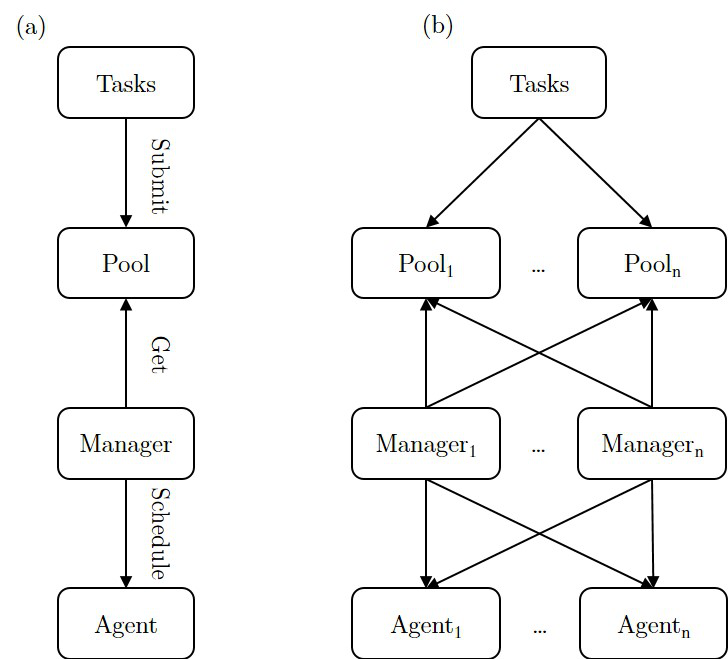
\includegraphics[width=0.45\textwidth]{figures/pilot_section3_1}
%   \caption{(a) Components and transitions of a generalized pilot
%     system; (b) Pilot systems may be composed of multiple
%     instances of the same components. \aznote{Bottom of figure
%         is slightly cut off}}
%   \label{fig:s3_pilot_diagram}
% \end{figure}

\jhanote{The question is what are the fundamental ``concepts''. It is
  not necessary that the concepts have a specific implementation or
  map to a component in \pilotjob system. As we know there are
  different ways in which tasks get committed to the \pilotjob
  system. One possible primary concept is that of logical grouping;
  all tasks are committed to a logical grouping -- where the grouping
  is such that all entities in this group will be executed
  (disregrarding details of how this grouping will happen, or who will
  perform the execution).  It appears that the concept of logical
  grouping of tasks is a fundamental one, and avoids a requirement of
  any further specification of of details of who/where/when; if so,
  then the notion of a pool can be dispensed with, which will have the
  advantage of liberating us from the requirement of imposing on the
  the manager the need to push/pulling tasks from a pool.}

% \mtnote{Different pool implementations, ways to make tasks available
%   to the manager: potential topics to discuss in Section 4?}

% Functionally, a pilot is a system that allows for a user to gain exclusive - i.e. not shared - control over the scheduling and execution of her tasks. As shown in Figure~\ref{fig:s3_pilot_diagram}, users submit tasks to a `pool', a store where tasks are collected and made available to a manager. 
% \onote{the more I think about it, the less I am convinced that we need the notion of a pool here. It's an implementation detail that might not
% even be part of every PJ implementation. It is not important when describing a PJ.}
% The implementation of a pool varies among \pilotjobs\onote{-Systems} with the pool being a stand-alone component or a subsystem of a master
% \onote{what is 'master'?}, and storing only the state of tasks or having also a dedicated set of capabilities.

\mtnote{Vocabulary: manager}
\mtnote{Capabilities across different manager implementations: potential topic to discuss in Section 4?}

Within a pilot system, a manager is responsible for getting tasks from
one or more pools and scheduling them into possibly multiple agents
(Figure~\ref{fig:s3_pilot_diagram}). Managers can offer a vast array
of capabilities and they greatly differ among \pilotjob
implementations. Scheduling algorithms but also mechanisms to allocate
dynamically resources to each task depending on availability and
performance evaluations are typical examples of capabilities already
offered, or potentially implementable, in this type of managers.

\mtnote{Vocabulary: agent}

Agents executes the tasks pushed by or pulled from one or more managers (Figure~\ref{fig:s3_pilot_diagram}). Clearly, an agent must have the right amount and type of resources for an appropriate extent of time in order to execute its tasks. As such, this requirement brings together pilots and jobs.

\mtnote{Vocabulary: Pilot Job}

A \pilotjob is a system that combines the conceptual constituents
defined for both `pilot' and `job' but also add the distinctive
concepts of `placeholder', `early binding' and `late binding' and
`multi-level scheduling'. \jhanote{we should consider a diagram to
  help distinguish late and early binding}

\mtnote{Vocabulary: Placeholder}

In order to get resources, each agent - or group of agents - of a
pilot system is scheduled by a user \onote{false. In the glideinWMS
  this is not done by the user} as a job within a given
infrastructure. These jobs are eventually granted the requested amount
of resources for the indicated period of time and their agents are
executed. At this point, an agent becomes a placeholder for the set of
resources that have been specified by and assigned to its job.
\onote{not convinced that we need a formal definition of
  'placeholder'.}

\mtnote{How different \pilotjob implementations deal with the
  peculiarities of the job submission system of different
  infrastructures; whether \pilotjobs implementations offer
  job-submission interoperability among different infrastructures:
  potential topics to discuss in Section 4?}

The submission process of agents depends on the capabilities exposed
by the submission system of the targeted infrastructure. For example,
users may or may not explicitly indicate a destination for where these
jobs need to be scheduled, may have to use dedicated queues and may
have to deal with limitations on what processes can be executed on a
specific infrastructure. Particularly important in this context are
networking capabilities as, without connectivity, agents would not be
able to communicate with their managers and, ultimately, with the end
users.

Once one or more placeholders become available on the given
infrastructures, users can start to use a \pilotjob system to execute
their tasks. Users own the placeholders and can run their tasks by
means of the corresponding agents without having to deal with the job
submission system of the infrastructure. \jhanote{Is is necessary that
  users ``own'' the agents. can the manager not own the placeholder?}

\mtnote{Vocabulary: multi-level scheduling}
\mtnote{Different ways to implement task scheduling: potential topics to discuss in Section 4?}

Tasks are scheduled on the available placeholders by means of a
dedicated scheduler, the pilot master or directly by the users
depending on the \pilotjobs implementations. As at least two level of
scheduling are involved - the one used to schedule the placeholders
and the other used to schedule tasks on the placeholder - \pilotjobs
are said to implement `multi-level scheduling' [ref] by means of
scheduling overlay [cit].

\mtnote{Vocabulary: binding} 

\mtnote{Binding capabilities; execution model: potential topics to
  discuss in Section 4?}

\jhanote{what is the general concept in the following? It is very
  focussed on specifics if not implementation details..}
Users partition the resources managed by means of a placeholder,
including its time allocation, so to execute multiple tasks in
parallel or sequentially. As the tasks require less time to complete
than the total walltime assigned to the placeholder, users never incur
in the overheads imposed by the job submission system of a given
infrastructure. The resources of multiple placeholders may also be
used at the same time so to achieve elaborated execution patterns. As
usual, the flexibility of a \pilotjob execution model depends on the
details of its implementation.


\mtnote{Vocabulary: early/late binding}
\mtnote{Late-binding capabilities: potential topics to discuss in Section 4?}

\jhanote{For ease of readability, we should make explicit the
  difference between binding and scheduling here.}  The act of
assigning resources to tasks is called `binding'. Note how 'binding'
is defined in contrast to scheduling.  \jhanote{I have brought the
  above sentence down here. I think for ease of readability, once we
  start discussing binding we should continue onto early and late
  binding. ALso in the definition of early and late binding, we should
  IMHO explicitly use the concept of ``when'' a task is bound to a
  resource in order for it to be concrete.}  The control exercised by
the users on their placeholders depends on the amount of information
they include when submitting their tasks to a pool. Users may fully
specify how and where a task should be executed or may leave the
manager and agents to evaluate those parameters for them. The former
is called `early binding' as users decide in advance how and where to
execute their tasks, the latter is called `late binding' because, at
submission time, how and where a task will be executed is unspecified.

Late binding requires specific capabilities. Manager(s) and agent(s)
must be able to evaluate the requirements of the submitted tasks and
maximize the efficiency of their binding depending on the peculiar
properties, configuration and state of the resources made available
through the placeholder(s). As such, in a late binding scenario,
managers and agents may decide the amount of placeholders to use, the
granularity of their partitions, the amount and type of the resources
to allocate to the tasks and where such tasks should be executed. In
an ideal late binding situation, users would be free only to specify
high-level, resource-independent parameters for their tasks as, for
example, the amount of time or money that should be spent for their
execution. 

% \subsection{Different components of the Landscape}

% \mtnote{The idea is to focus this subsection on the relationship between \pilotjob and the environment - re infrastructure - where its agents are scheduled and executed. The analysis should focus on the set of capabilities that pertain exclusively - at least in theory - to each domain. This would outline functionally and qualitatively the `landscape' of \pilotjob and offer a base for the critical analysis of the \pilotjobs implementations in \S 4. The idea would be to show how implementations choose ad hoc solutions depending on the specific characteristic of their landscape, both in terms of compensating for their limitations or exploiting their peculiarities. }

% \begin{itemize}

%     \item Resource Types

%         \begin{itemize}
%             \item HTC Grids
%             \item HPC Grids
%             \item Virtualized Environments (Clouds)
%             \item Hybrids, Cloud-bursting, etc.
%         \end{itemize}

%     \item Organizational Structures

%         \begin{itemize}
%             \item Virtual Organizations
%             \item "The XSEDE Model"
%         \end{itemize}

%     \item Software and Services \mtnote{this subsection would focus specifically on this item}

%         \begin{itemize}
%             \item Single-site, local workload mgmt. systems (HPC schedulers)
%             \item Single-site endpoint services (e.g., GRAM, CREAM)
%             \item Multi-site workload mgmt. systems (meta-scheduler)
%             \item File transfer services
%             \item Metadata services
%         \end{itemize}

%     \item Access Mechanisms

%         \begin{itemize}
%           \item API 
%             \item CMD Line tools
%             \item Gateways (web)
%         \end{itemize}

%     \item Applications and Use-Cases

%         \begin{itemize}
%             \item X
%         \end{itemize}

% \end{itemize}

% \jhanote{Something akin to Matteo's diagram}

% %\begin{itemize}
% %        \item PJ abstractions are not defined in a void;
% % \item use cases, scientific practice and distributed applications;
% %        \item heterogeneous DIs: grid, cloud and hybrids;
% % \item jobs and services;
% %        \item LoAs implied by the PJ abstractions;
% % \item diagram.
% %\end{itemize}
% %
% \subsection{Common Terms and Definitions}

% \alnote{What to do with the terms, such as many-task computing, meta computing, grid computing, etc.? It might make sense to couple the evolution of \pilots to the evolution of these infrastructure paradigms (hypes). Maybe in history section.}

% \mtnote{I think subsection 3.0 addresses this comment. If we all agree on todays call, I will comment out the entire subsection.}

% \alnote{Can we start of with the P* elements so that we have something?}
% \begin{itemize}
%     \item application
%     \item workflow
%     \item pilot framework
%     \item manager
%     \item pilot, agent, executor, butler process, placeholder
%     \item scheduler
%     \item job
%     \item workload
%     \item ensemble
%     \item \computeunit
%     \item platform
% \end{itemize}

% \mtnote{Following AndreL suggestion. Work in progress, I am still trying to map this list into \S2 + P*. The final version of the diagram will be based on these lists.}
% \begin{itemize}
%     \item Common concepts
%         \begin{itemize}
%              \item Placeholder
%              \item $\langle$Late binding/placement$\rangle$
%              \item $\langle$Master/worker$\rangle$
%              \item Workload
%              \item Job
%              \item \computeunit
%         \end{itemize}
%     \item Distinctive concepts
%         \begin{itemize}
%              \item $\langle$High-level framework$\rangle$
%              \item Workflow
%              \item Scheduler
%              \item Ensemble?
%         \end{itemize}
% \end{itemize}

%The terminology used to describe the implementations of pilot-job reviewed in
%section 2 varies depending not only on the type of implementation considered --
%simple/core, pilot-based scheduling and higher-level application framework --
%but also on the application domain where they are deployed and leveraged.
%Nonetheless, some common concepts can be identified so that a common vocabulary
%can be developed. The goal is to leverage such a vocabulary to ...
%\mtnote{what exactly do we want to achieve with Section 4?}.

%'Late-binding' is one of the concepts that persist unchanged across all the
%pilot-job implementations. 
%\begin{itemize}
%        \item Late-binding: 
%\end{itemize}
%
%The very same nature of pilot-job is that of enabling a late-binding of
%resources to jobs. This is what allows for a pilot-job to offer 'load
%balancing', 'scheduling' and to some extent 'domain distribution'. Late-binding
%is also directly related to the possibility for a pilot-job system to fulfil
%the qualitative requirements related to the efficiency with which jobs are
%distributed, scheduled and executed by the user on one or more distributed
%infrastructure. \mtnote{shall we assume these definitions? I think so but I
%want to be sure.}

%% \newpage

%% \begin{table*}[t]
%%   \footnotesize{
%%  \up
%%  \centering
%%  %\begin{tabular}{|p{2.5cm}|p{3cm}|p{3cm}|p{3cm}|p{3cm}|p{3cm}|p{3cm}|}
%%  \begin{tabular}{|p{2cm}|p{2cm}|p{2cm}|p{2cm}|p{2cm}|p{2cm}|p{2cm}|}
%%   \hline
%%   \textbf{Pilot Element}
%%   &\textbf{BigJob} &\textbf{DIANE} &\textbf{Condor-G/Glide-in} &\textbf{Swift/Coaster} &\textbf{Bosco} &\textbf{GWPilot}\\
%%   \hline
%%   Pilot-Manager &BigJob Manager & RunMaster & condor\_master, condor\_collector, condor\_negotiator, condor\_schedd &Coaster Service & Condor & Gridway\aznote{fill in}\\ 
%%   \hline
%%   \pilot &BigJob Agent  & Worker Agent &condor\_master, condor\_startd &Coaster Worker & condor\_master, condor\_startd& GWpilot\aznote{(?) check} \\
%%   \hline
%%   \computeunit  \ (CU) &Task &Task &Job &Application Interface Function (Swift Script) & Job & Task\\
%%   \hline
%%   \su \ (SU) &Sub-Job &Task &Job &Job & Job & Task \\
%%   \hline
%%   Data support & BigData& & & & &\\
%%   \hline
%%   Deployment (centrally hosted vs application)  & Application & & & &Runs locally, requires remote cluster install & Centrally hosted \aznote{Req. gridway install}\\
%%   \hline
%%   Interoperable & via SAGA & & & &Yes, via Condor & Yes, via BLAHPD\\
%%   \hline
%%   Abstraction(?) & & & & & &\\
%%   \hline
%%   Coordination(?) &Advert & & & & &\\

%% % \hline
%% % Dynamic Resources &no/yes &yes (AgentFactories)\\
%%  \hline
%%  \end{tabular}
%%  \caption{\textbf{Comparing PJ Systems} 
%%    Exposing the commonalities of PJ systems \aznote{Some of these are going to be almost identical e.g. Bosco w/
%%      Condor -- combine their columns to emphasize similarity?} \aznote{properly formatted later once complete/judged relevant}
%%    \aznote{Not sure of relevance of an ``all-encompassing table'' if we are
%%      going to be focusing on ``landmark'' Pilot-Job systems...
%%      put this on the back-burner for the time being..}
%%  \up
%%  } 
%%  \label{table:bigjob-saga-diane}
%% }
%% \end{table*}


%% \begin{landscape}
%% \begin{table}
%% \begin{center}
%% \begin{footnotesize}
%% \begin{tabular}{|p{3.0cm}|p{3.5cm}|p{2.3cm}|p{1.9cm}|p{3.7cm}|p{2.5cm}|}
%% \hline {\bf BigJob}
%% & {\bf Diane}
%% & {\bf Condor/Glide-in}
%% & {\bf Swift}
%% & {\bf Bosco}
%% & {\bf GWPilot}
%% \\
%% \hline

%% Montage
%% & Multiple sequential and parallel executables
%% & Files
%% & Dataflow (DAG)
%% & Dynamic process creation, workflow execution, file transfer
%% & test
%% \\
%% \hline

%% \end{tabular}
%% \end{footnotesize}
%% \caption{\label{Tab:AppChars} }
%% \end{center}
%% \end{table}
%% \end{landscape}

\section{Pilot-Job Systems Revisited}
\aznote{Ashley's section}
Despite the apparent diversity in existing \pilotjobs,
they can be reduced to a set of common functionality and
discussed as such via use of the the terminology presented
in \S\ref{sec:vocab}.
%has implications
%for the interoperability of existing and future \pilotjobs, and
%lends insight into the design and usage of \pilotjob systems.
% application design to enhance job/data(?)
%mobility, management, and potential run-time responsiveness via
%late-binding/etc.  
We will see that throughout the evolution
of the \pilotjob concept, several core concepts have remained stable
while new additions enhance cross-platform interoperability,
ease of usage and deployment, and incorporate the ability to
schedule data as well as jobs.   These additions illustrate
the flexibility and power of \pilotjobs, and emphasize the
need for a common vocabulary/treatment to describe the
developing landscape.

\jhanote{Ashley to ``finish'': AppLeS, MyCluster and PANDA: Ole to
  finish Glide-in, Corral and Bosco: Mark to finish DIANE,
  Swift/falkon, DIRAC(?)}

\aznote{Should we organize this section in order of when the PJ-systems
were released?}

\subsection{Comparing \pilotjobs via a Common Framework \& Vocabulary}
\aznote{Suggest removing the subsection header; making individual
pilotjobs into subsections instead?  Unless we decide to include
another subsection in here -- but in that case, do not want to overlap
with the conclusion}
In light of the common vocabulary discussion in 
\S\ref{sec:vocab}, a representative set of \pilotjobs
has been chosen for further analysis.  

At least one \pilotjob from each categorization in
\S\ref{sec:survey} is analyzed via a common
vocabulary, allowing for a standard
``baseline'' of each \pilotjob categorization to be
examined.  Examining these \pilotjobs via a
common vocabulary exposes their core similarities, and allows a
detailed analysis of their differences.

%Representative \pilotjobs from each \pilotjob category
%in Section~\ref{sec:survey} are chosen and compared within
%the bounds of that category, illustrating the core similarities
%between the Pilot-Jobs in a given category.

\textit{Finally, we perform
a cross-cutting analysis, demonstrating that across the categorical
distinctions all approaches remain true ``\pilotjobs'' with regard
to their base functionality.  The segmentation between categories
is exposed to reveal why \pilotjobs have evolved to have
differing capabilities, with the end-goal being a
complete understanding of the \pilotjob ecosystem via a common
vocabulary.}
\aznote{Maybe this is better-suited for the conclusion?}

%\subsubsection{Condor-G}
%% \aznote{Section copied and pasted from IPDPS paper for now -- plan
%% to use this general sort of information + reword using our spiffy 
%% vocabulary presented in this paper}
%% Condor-G pioneered the Pilot-Job concept~\cite{condor-g}. The pilot is
%% actually a complete Condor pool that is started using the Globus
%% service of a resource. This mechanism is referred to as Condor
%% Glide-In. Subsequently, jobs can be submitted to this Glide-In pool
%% using the standard Condor tools and APIs. Condor utilizes a
%% master/worker coordination model. The PJ manager is referred to as the
%% Condor Central Manager. The functionality of the Central Manager is
%% provided by several daemons: the condor\_master that is generally
%% responsible for managing all daemons on a machine, the
%% condor\_collector which collects resource information, the
%% condor\_negotiator that does the matchmaking and the condor\_schedd
%% that is responsible for managing the binding and scheduling
%% process. Condor generally does not differentiate between workload,
%% i.\,e.\ WU, and schedulable entity, i.\,e.\ SU. Both entities are
%% referred to as job. However, it supports late binding, i.\,e.\
%% resources a job is submitted to must generally not be available at
%% submission time. The scheduler matches the capabilities required by a
%% WU to the available resources. This process is referred to as
%% matchmaking. Further, a priority-based scheduler is used. For
%% communication between the identified elements Condor utilizes
%% point-to-point messaging using a binary protocol on top of TCP.

%% Different fault tolerance mechanisms, such as automatic retries, are
%% supported.  Further, Condor supports different security mechanisms:
%% for authentication it integrates both with local account management
%% systems (such as Kerberos) as well as grid authentication systems such
%% as GIS. Communication traffic can be encrypted.


\begin{table*}[t]
 \up
 \centering
 \begin{tabular}{|p{3cm}|p{3.2cm}|p{3cm}|p{3cm}|p{3cm}|}
  \hline
  \textbf{Pilot-Job System} &\textbf{Pilot (Resource) Provisioning}    &\textbf{Job-to-Resource (Pilot) Binding}  &\textbf{Single-/Multi-User Pilots} &\textbf{Classifier IV}  \\
  \hline
          AppLeS            & N/A                                      & Automatic (algorithmic/profiling)  & Single (?) & --                     \\ 
  \hline
          MyCluster         & Manual, Explicitly User-controllable     & Manual                             & Single (?)                  & --                     \\ 
  \hline
          PanDA             & Automatic, Not user-controllable         & Manual(?)                          & Single (?)  \aznote{\url{http://indico.cern.ch/getFile.py/access?contribId=2&sessionId=6&resId=0&materialId=slides&confId=45473} says otherwise, but I don't think so...}    & --                     \\ 
  \hline
          GlideinWMS        & Automatic, Not user-controllable         & Manual (rule-driven) / Automatic   & Multi / Single (via Corral) & --                     \\ 
  \hline
          SWIFT/Coaster     & --                                       & --                                 & --                          & --                     \\ 
 \hline
          BoSCO             & Manual, Explicitly User-controllable     & Manual (rule-driven) / Automatic   & Multi / Single              & --                     \\ 
 \hline
          BigJob             & Manual, Explicitly User-controllable     & Manual (rule-driven) / Automatic   & Single              & --                     \\ 
 \hline
 \end{tabular}
 \caption{\textbf{Different pilot-job systems and their key. 
 \onote{Possible classifiers:
 user/system space: can pilots be controlled from system / user space. TODO:
 discuss why we chose specific classifiers!}}
 \up} 
 \label{table:bigjob-saga-diane}
\end{table*}


% -----------------------------------------------------------------------------
%
\subsubsection{AppLeS}

\textcolor{green}
{
\textbf{Structure}
\begin{itemize}
\item Functional description: core components -- X does that, Y does that, Z doest that.
\item What applications were they designed for?
\end{itemize}
}

\textcolor{red}
{
\textbf{Usage of 'relevant' terms from section three}
\begin{itemize}
\item Term 1 =
\item Term 2 =
\end{itemize}
}

\textcolor{blue}
{
\textbf{Mapping to table 1:}
\begin{itemize}
\item Pilot (Resource) Provisioning:
\item Job-to-Resource (Pilot) Binding:
\item Singe-/Multi-User pilots:
\end{itemize}
}

AppLeS is a \textit{pre-pilot} framework which allows software built using it to take advantage
of enhanced scheduling and resource selection capabilities.
With AppLeS, application-level scheduling and resource selection are handled by a
per-application \texttt{AppleS agent}.
%\aznote{AppLeS agent covers resource discovery, resource selection,
%  schedule generation, schedule selection, application execution,
%  and schedule adaptation}
An \texttt{AppLeS agent} roughly handles the \pilotjob functionality contained in
\textit{\pilotjob agents} and \textit{managers}.  This includes resource
selection, scheduling tasks to resources, and managing application execution.
Job-to-Resource \textit{binding} is handled automatically via the AppLeS agent.
%.  In addition, an incomplete subset of
%\pilotjob functionality such as application-scheduling is present in AppLeS.
AppleS also contains features not fundamental to the \pilotjob paradigm, such
as resource discovery via Grid resource discovery services and peformance
modelling for resource selection.  The entire package thereby reduces the
complexity of assigning tasks to resources from the user's point of view
and enables applications to run in a more adaptive fashion.

The lack of a \textit{placeholder job} limits the functionality 
of application-level scheduling, as tasks
must wait in unpredictable resource manager queues before being executed,
undermining the level of control.  For this reason, AppLeS
is not a ``true'' \pilotjob system, as a \textit{placeholder}
is required to enable fundamental \pilotjob functionality such as
\textit{multi-level scheduling.}
However, AppLeS has still been used to choose destinations
for satellite image files, optimize the execution of data-parallel matrix
calculations, distribute computational biology genetic searches 
across resources with varying response/availability times, and
analyze biochemical interactions while dynamically recreating
schedules to account for changes in performance predictions.
\aznote{Previous sentence to satisfy request for \pilotjob
domain usage}
\aznote{Should I put something here like 
``AppLeS has been successful in these domains due in part
to the usefulness of the M-W paradigm which \pilotjobs
are based on, but the following ``True'' \pilotjobs
illustrate the extended reach/power made available
through a proper \pilotjob approach''?}

%% \aznote{Lack of multi-level scheduling asserted because even
%% though AppLeS allows for application-level scheduling,
%% it is still submitted to usual resource manager queues, not an internal
%% ``pilot'' queue}
%% Such enhancements
%% are made in the ``true'' \pilotjob systems which succeed it,
%% offering additional adaptibility and user-control over that
%% made possible by AppLeS.
\aznote{Early vs. late binding here -- I am not sure.  AppLeS generates
a task-resource mapping early before jobs are even running + then sticks 
to it making it ``early binding'' in my mind,
even though it does so after profiling the application.  However, according
to the vocab, if the manager/agents choose which resources will be used
it's ``late binding''.  So that is what I will go with.}

%\aznote{\url{http://www.sc2000.org/techpapr/papers/pap.pap169.pdf} - Also consider this paper:
%The AppLeS Parameter Sweep Template: User-Level Middleware for the Grid?}

% -----------------------------------------------------------------------------
%
\subsubsection{MyCluster}

\textcolor{red}
{
\textbf{Mapping to section 3:}
\begin{itemize}
\item Term 1 =
\item Term 2 =
\end{itemize}
}

\textcolor{blue}
{
\textbf{Mapping to table 1:}
\begin{itemize}
\item Pilot (Resource) Provisioning:
\item Job-to-Resource (Pilot) Binding:
\item Singe-/Multi-User pilots:
\end{itemize}
}

%% \aznote{NOT EVEN SURE THIS IS A ``BASIC PILOT-JOB SYSTEM'' right now:
%% ``Our system delegates the responsibility of submitting the
%% job proxies to a single semi-autonomous agent spawned,
%% through Globus, at each TeraGrid site during a virtual login
%% session. This agent translates the job proxy submission to the
%% local batch submission syntax, maintains some number of job
%% proxies throughout the lifetime of a login session, and may
%% negotiate migration of job proxies between sites based on
%% prevailing job load conditions across sites.''
%% Rather, it looks like MyCluster provides some method of 
%% submitting jobs to resources in a unified manner, much like
%% AppLeS.  When it comes time for the job to run, however,
%% it must wait in the local queuing system...?  In short,
%% looks like abstraction across multiple resources with some
%% functionality to handle everything from a single unified
%% access point including data handling, but
%% there is no concept of a placeholder/agent.
%% }

%% \aznote{I still agree with my above statements after additional reading --
%% it looks like this is kind of a ``virtualization'' system for grids
%% where you can submit/monitor jobs via a centralized interface and lacking
%% in what we consider vital to be a full-fledged Pilot-Job system.  Would
%% welcome discussion here.}

MyCluster is a \textit{basic \pilotjob system} which is a direct
abstraction of cluster-based distributed computing systems.
%% The stated goal of the project is to 
%% ``build personal [...] clusters on demand''
%% \aznote{from webpage} and in doing so
%% inadvertantly implements \pilotjob functionality to accomplish
%% its aims.
The authors describe their system
as a ``personal cluster'' with the goal of achieving on-demand,
user-schedulable computational resources aligning closely with what is
provided by our more formal definition of \pilotjobs.

MyCluster implements several \pilotjob analogues: the \texttt{Master
  Node Manager}, which acts as a \textit{\pilotjob Manager}, the
\texttt{Task Manager}, which acts as an \textit{\pilotjob Agent},
\texttt{Job Proxies}, which act as \textit{placeholders}, and
\texttt{Slave Node Managers}, which handle (are?) \textit{\pilotjob
  \cus}.  Both resource provisioning and job-to-resource \textit{bindings}
are handled manually by the end user.
The end result is a complete \textit{basic \pilotjob system}, despite the
authors of the system being constructed not having used the word ``pilot''
once!~\cite{1652061}  

Additional features above and beyond the \textit{basic \pilotjob system}
concept include: the inclusion of a MyCluster
\texttt{virtual login session}, which
is commandline interface designed to allow users to interactively
monitor the status of their \textit{placeholders} and \textit{\cus};
the automatic recovery of placeholders after loss due to exceeding wallclock
limitations or node reboots; and authentication of all TCP
connections used in the system via 64-bit key encryption and
GSI authentication mechanisms.

MyCluster was designed for and successfully executed on NSF TeraGrid
resources, enabling large-scale cross-site submission of ensemble
job submissions via its virtualized cluster interface.  
This approach makes the \textit{multi-level scheduling} abilities
of \pilotjobs explicit; rather than directly \textit{binding}
to individual TeraGrid resources, users allow the virtual grid
overlay to \textit{schedule} tasks to multiple allocated TeraGrid sites
as a whole.
 
%\textit{Manager} functionality is handled by MyCluster's 
%\texttt{Master Node Manager}.

%% Shortcomings include ...  (lack of heterogenous support?)

%% \begin{itemize}
%% \item Master Node Manager = Manager \aznote{Master Node
%% Manager process within a GNU Screen session that then
%% starts the Condor/SGE master daemons in user space if
%% needed.}
%% \item Agent Manager \aznote{ The
%% agent manager remotely executes a Proxy Manager process at
%% each participating site using Globus GRAM}
%% \item Submission Agent -- \aznote{Wrapper for GridShell, wraps
%%   multiple grid resources to a single ``virtual'' cluster
%% \url{https://www.opensciencegrid.org/bin/view/Interoperability/GridShellEvaluation}}
%% \item Proxy Manager = one at each site, reports back to central
%%   agent manager w/ heartbeat to keep awareness of resource state
%% \item Task Manager = \textit{agent}
%% \item Slave-node managers = compute units (?) (probably not,
%%   barely mentioned in the paper)
%%   \aznote{The slave node managers are responsible for starting the
%%     Condor or SGE job-starter daemons. These daemons connect
%%     back to the master processes on the client workstation, or to a
%%     pre-existing departmental cluster, depending on the virtual
%%     login configuration.
%%   }
%% \item Job proxy (?)
%% \end{itemize}

% -----------------------------------------------------------------------------
%
\subsubsection{PanDA}

\textcolor{red}
{
\textbf{Mapping to section 3:}
\begin{itemize}
\item Term 1 =
\item Term 2 =
\end{itemize}
}

\textcolor{blue}
{
\textbf{Mapping to table 1:}
\begin{itemize}
\item Pilot (Resource) Provisioning:
\item Job-to-Resource (Pilot) Binding:
\item Singe-/Multi-User pilots:
\end{itemize}
}

PanDA's \textit{manager} is called a \texttt{PanDA server}, and matches
jobs with \pilots in addition to handling data management.
PanDA's \textit{\pilot}
is called, appropriately enough, a \texttt{pilot}, and handles the execution
environment.  These pilots are generated via PanDA's \texttt{PilotFactory},
which also monitors the status of pilots.
Pilot-resource \textit{provisioning} is handled by PanDA itself and is not 
user-controllable, whereas job-to-resource \textit{binding} is handled
manually by users.
This basic functionality (pilot creation and management) provides 
PanDA with all of the baseline capabilities required for a \pilotjob.

As PanDA is an \textit{Advanced \pilotjob System}, it enables functionality
beyond that of a \textit{Basic \pilotjob}.
PanDA contains some additional backend features such as \texttt{AutoPilot}, which
tracks site statuses via a database, and \texttt{Bamboo} which adds
ATLAS database interfacing.  Enhancements to the userspace include 
\texttt{Monitor}, for web-based monitoring, and the \texttt{PanDA client}.
\texttt{PanDA Dynamic Data Placement} \cite{maeno_pd2p:_2012} 
allows for additional, automatic data
management by replicating popular input data to underutilized resources
for later computations.

PanDA was developed to provide a \pilotjob system for ATLAS which could
handle large numbers of data-driven processing workloads.  Having proven itself
capable in this role, it has also been used for other projects such
as the Open Science Grid.  This illustrates the importance of designing
\pilotjobs which are easily adaptable such that \pilots are not tied
to any particular DCI; in this manner, their advantages can be made
available beyond their original design scope.
%\aznote{Discussion on PanDA's design for LHC data processing and why \pilotjobs
%work for this, or is this out-of scope?}


%% \textbf{job, task, resource, infrastructure, scheduling, pilot, pool, manager,
%%   agent, Pilot-Job, placeholder, multi-level scheduling, binding, early/late
%%   binding}

%% \begin{itemize}
%% \item Based upon Condor-G/Glidein, uses multiple queues
%% \item Jobs submitted via Condor-G
%% \item Jobs run with wrappers, on worker nodes they download/execute PanDA pilot code
%% \item Pilot then asks for job that worker node can handle
%% \item Stages in input files; executes and monitors progress of job; stages out output;
%%   cleans up environment
%% \item ``Special Features''
%%   \begin{itemize}
%%   \item Job/disk monitoring
%%   \item Job recovery (leaves output files resident for another 
%%     process to resume from)
%%   \item Multi-job processing (submit batch of jobs to a single pilot)
%%   \item Certificate/token-based security
%%   \item gLExec security (user's identity used instead of Pilot credentials)
%%   \end{itemize}

%% \item PanDA server (task buffer -- job queue manager keeps track of
%%   active jobs, brokerage -- matches jobs  with sites/pilots and manages
%%   data placement, job dispatcher -- receives requests from pilots and sends
%%   jobs payloads, data service -- dispatch and retrieval from sites)
%% \item PanDA DB (general DB = advert?)
%% \item PanDA client (user client for submission/etc)
%% \item Pilot (execution environment)
%% \item AutoPilot (pilot submission, management, monitoring), submits
%%   pilots to remote sites and tracks site status via database
%% \item SchedConfig (configuration database)
%% \item Monitor (Web-based monitoring)
%% \item Logger (logs incidents w/ Python logging)
%% \item Bamboo (interface w/ ATLAS database)
%% \item PilotFactory -- generates pilots (sends schedd glideins to remote sites)
%%   and monitors pilot status, basically enables use of glideins with PanDA (?)
%% \end{itemize}



% -----------------------------------------------------------------------------
%
\subsubsection{HTCondor GlideinWMS}

\textcolor{red}
{
\textbf{Mapping to section 3:}
\begin{itemize}
\item Term 1 =
\item Term 2 =
\end{itemize}
}

\textcolor{blue}
{
\textbf{Mapping to table 1:}
\begin{itemize}
\item Pilot (Resource) Provisioning:
\item Job-to-Resource (Pilot) Binding:
\item Singe-/Multi-User pilots:
\end{itemize}
}

\textit{Collectors} are the managers, with one collector per
GlideinWMS system.
\textit{Glidein factory daemon}s are responsible for
submitting pilot jobs to grid pools\aznote{Use diff vocab for grid pool?}.
They therefore correspond to pilot managers.
\textit{VO frontend daemons} are the schedulers, which map jobs
to pilots.  GlideinWMS takes advantage of late-binding, as
jobs are not selected for resources until the pilots start.\aznote{This
should be true of all systems described in this section -- do we
need to explicitly say so for each pilot system?}
\textit{WMS collector machine} manages communication between the glidein
factory daemons(pilot managers) and VO frontend daemons(schedulers)
and so corresponds to \aznote{We don't have anything for this.  This
sounds like what REDIS/etc do for BJ though.  Should we incorporate this
into our vocabulary?}
\textit{User jobs} correspond to compute units \aznote{Right?}

\begin{itemize}
%Unlisted things \\
\item Workflow (doesn't seem to be explicit support)
\item Workload (is this just a list of user jobs that are queued up)
\item Placeholder (isn't this the same kind of deal as a Pilot-Job/PJ
waiting in a queue?)
\item Pilot framework (The entire GlideinWMS qualifies as a ``pilot
framework'', correct?)
\item Ensemble \aznote{How to tie this in}
\item Platform \aznote{Ditto}
\item Master-Worker \aznote{Likewise, we could say that the
VO factory daemons are the masters with the pilots the workers,
but this seems overly pedantic?}
\end{itemize}

\textbf{CorralWMS:} CorralWMS is an alternative front-end for GlideinWMS-based
infrastructures. It replaces or complements the regular GlideinWMS front-end
with an alternative API which is targeted towards workflow execution. Corral was
initially designed as a standalone pilot (glidein) provisioning system for
the Pegasus workflow system where user  workflows often produced workloads
consisting of many short-running jobs as well as mixed workloads consisting of
HTC and HPC jobs.

Over time, Corral has been integrated into the GlideinWMS stack as CorralWMS.
While CorralWMS still provides the same user-interface as the initial, stand-
alone version of Corral, the underlying pilot (glidein) provisioning is
now handled by the GlideinWMS factory.

The main differences between the GlideinWMS and the CorralWMS front-ends lie in
identity management and resource sharing. While GlideinWMS pilots (glidins) are
provisioned on a per-VO base and shared / re-used amongst members of that VO,
CorralWMS pilots (glideins) are bound to one specific user via personal  X.509
certificates. This enables explicit resource provisioning in non-VO centric
environments, which includes many of the HPC clusters that are part of U.S.
national cyberinfrastructure (e.g., XSEDE).


% -----------------------------------------------------------------------------
%
%\subsubsection{Corral}
%\onote{Corral seems to be a component in the glidein-WMS landscape and 
%not an independent pilot-job implementation. I don't think that we should 
%dedicate an extra section to it.}
%\aznote{SJ asked for an investigation of Corral -- not sure that this
%deserves a full analysis at this point on a technical level despite
%being commonly used, open to suggestions}

%Corral is designed to allow hybrid HTC/HPC execution, in which
%many small jobs may be executed in conjunction with larger runs. 
%\cite{Rynge:2011:EUG:2116259.2116599}
%\aznote{Back this up w/ paper refs -- paper is somewhat dated,
%verify this is still true today}.  Corral operates as a Glidein
%WMS frontend\aznote{main reason that I think we shouldn't include
%Corral in its own section...}, where GlideinWMS manages the size
%of Condor glide-in pools.
%\begin{itemize}
%\item Workflow - handled by Pegasus workflow management system
%  \aznote{True in the paper I am using, but not handled by Corral itself, so should we include this?}
%\item Placeholder - handled by multislot requests 
%  \aznote{multislot request requests a single large
%    GRAM job, and then starts glideins within this container}
%\item Job
%\item Compute unit
%\item Workload 
%\item Will fill this in later...
%\end{itemize}


% -----------------------------------------------------------------------------
%
\subsubsection{Coasters}

\textcolor{red}
{
\textbf{Mapping to section 3:}
\begin{itemize}
\item Term 1 =
\item Term 2 =
\end{itemize}
}

\textcolor{blue}
{
\textbf{Mapping to table 1:}
\begin{itemize}
\item Pilot (Resource) Provisioning:
\item Job-to-Resource (Pilot) Binding:
\item Singe-/Multi-User pilots:
\end{itemize}
}

\msnote{Main coasters ref: http://www.ci.uchicago.edu/swift/papers/UCC-coasters.pdf}

The Coaster System (or "Coasters") is a Java CoG based Pilot-Job system
created for the needs of the Swift parallel scripting language.

Coasters was designed to both usability and performance goals.


\textit{Coaster Service} is deployed on remote clusters.

\textit{Coaster Client} is deployed locally.
\textit{Coaster Workers} 



% -----------------------------------------------------------------------------
%
\subsubsection{BigJob}

\textcolor{red}
{
\textbf{Mapping to section 3:}
\begin{itemize}
\item Term 1 =
\item Term 2 =
\end{itemize}
}

\textcolor{blue}
{
\textbf{Mapping to table 1:}
\begin{itemize}
\item Pilot (Resource) Provisioning:
\item Job-to-Resource (Pilot) Binding:
\item Singe-/Multi-User pilots:
\end{itemize}
}

In the BigJob framework, a \pilot is, appropriately enough, called a
\pilot. The BigJob \textit{manager} is called a \textit{\pilot
  Manager}, which is the central coordinator of the
framework. \jhanote{Which is the general concept? I think
  Pilot-Manager is the general concept and BigJob-Manager a specfic
  realization of it} The \textit{\pilot-Manager} is responsible for
the orchestration and scheduling of \pilots. It runs locally on the
machine used to initiate the distributed application which may or may
not be the same resource as the machine used on which the distributed
application executes.

The manager ensures that tasks are launched onto the correct resource
using the correct number of processes. The \pilot-manager submits a
\pilot to a remote resource's batch queueing system; when these
\pilots becomes active, a \textit{Agent} (of the manager, not of the
pilot) on the remote resource gathers information about its resource
and executes the actual tasks the resource. \jhanote{I don't think we
  should call it a pilot-agent, as it is agent of the manager not of
  the pilot. OK?}  Each resource has its own Pilot Agent.\jhanote{I
  don't think this is correct. Each pilot should contain an agent, not
  each resource} \jhanote{the separation of roles between the agent
  and the manager is unclear: does the agent do the mapping of tasks
  to the cores/nodes/processors or is that done by the manager?}

The communication between the Manager and Agent(s) is achieved through
the {\it Distributed Coordination Service}, which is most often a
database that stores information about jobs, information about the
jobs (executable, input data, etc.), and job status. These
functionalities comprise a set of baseline capabilities that
constitute a Pilot-Job.

BigJob extends the notion of a basic \pilotjob and offers user-level
control of \pilot placement as well as late-binding capabilities of a
\pilot to a remote resource. BigJob was designed to natively provide
support for MPI jobs, as well as work on a variety of back-end systems
by utilizing the Simple API for Grid Applications (SAGA) as its
backend. BigJob has been extended to work with data and, similarly to
\pilotjobs, abstract away direct user communication between different
storage systems. This makes BigJob extensible to both cloud and
heterogenous storage environments.

\subsubsection{DIANE}

\textcolor{red}
{
\textbf{Mapping to section 3:}
\begin{itemize}
\item Term 1 =
\item Term 2 =
\end{itemize}
}

\textcolor{blue}
{
\textbf{Mapping to table 1:}
\begin{itemize}
\item Pilot (Resource) Provisioning:
\item Job-to-Resource (Pilot) Binding:
\item Singe-/Multi-User pilots:
\end{itemize}
}

\aznote{Do we want to define single-user vs multi-user? 
  Communication methods?  Output aggregrator?}

\aznote{DIANE runmaster/etc not included in current paper we
have cited}

DIANE~\cite{Moscicki:908910} is a task coordination framework, which
was originally designed for implementing master/worker applications,
but also provides PJ functionality for job-style executions.
DIANE utilizes a single hierarchy of worker agents as well as a PJ \textit{manager}
referred to as \texttt{RunMaster}.  The manager creates
placeholders called \texttt{Workers}, which register with and receive jobs from the manager.
%For the spawning of PJs a separate script, the so-called submitter script, is
%required. 
The \textit{scheduler} for DIANE is known as the \texttt{Planner}.
%For the access to the physical resources the GANGA
%framework~\cite{Moscicki20092303} can be used.
%A worker agent generally manages only a single
%core and thus, by default is not able to run parallel applications.
% Once the worker agents are started they register themselves at the RunMaster.
% GANGA provides a
% unified interface for job submissions to various resource types, e.\,g.\ EGI
% resources or TG resources via a SAGA backend.
%DIANE operates on the master-worker computing model.

%The \textit{manager} for DIANE is called the \texttt{Master}, and contains
%the \textit{scheduler} for DIANE, which is known as the \texttt{Planner}.
%The manager creates placeholders called \texttt{Workers}, which
%register with and receive jobs from the manager.

The workflow is then such that a user submits a parallel job to
the grid using a DIANE client.  The client then creates the Pilot manager
and remains in contact with it to control its \pilotjobs.  Results
are aggregated through use means of the DIANE
\texttt{Integrator}.\aznote{No mapping vocab for the integrator as of now.}
DIANE includes a simple capability matcher and FIFO-based task scheduler
to help facilitate the execution of jobs.
Plugins for other workloads, e.\,g.\ DAGs or for data-intensive
application, exist or are under development. The framework is extensible:
applications can implement a custom application-level scheduler.

For communication between the RunMaster and
worker agents point-to-point messaging based on CORBA~\cite{OMG-CORBA303:2004}
is used. CORBA is also used for file staging.
DIANE is a single-user PJ, i.\,e.\ each PJ is executed with the
privileges of the respective user. Also, only WUs of this respective user can be
executed by DIANE. DIANE supports various middleware security mechanisms
(e.\,g.\ GSI, X509 authentication). For this purpose it relies on GANGA. The
implementation of GSI on TCP-level is possible, but currently not yet
implemented. Further, DIANE supports fault tolerance: basic error detection and
propagation mechanisms are in place. Further, an automatic re-execution of WUs
is possible.

DIANE is primarily designed with respect to HTC environments (such as
EGI~\cite{egi}), i.\,e.\ one PJ consists of a single worker agent with the
size of 1 core.

% -----------------------------------------------------------------------------
%
\subsubsection{BoSCO}

\textcolor{red}
{
\textbf{Mapping to section 3:}
\begin{itemize}
\item Term 1 =
\item Term 2 =
\end{itemize}
}

\textcolor{blue}
{
\textbf{Mapping to table 1:}
\begin{itemize}
\item Pilot (Resource) Provisioning:
\item Job-to-Resource (Pilot) Binding:
\item Singe-/Multi-User pilots:
\end{itemize}
}

BoSCO is a user-space job submission system based on HTCondor. BoSCO was
designed to allow individual users to utilize heterogeneous HPC and grid
computing resources through a uniform interface. Supported backends include PBS,
LSF and GridEngine clusters as well as other  grid resource pools managed by
HTCondor. BoSCO supports both, an agent-based (\textit{glidein} / worker) and
a native job execution mode through a single user-interface.

BoSCO exposes the same \textit{ClassAd}-based user-interface as HTCondor,
however, the backend implementation for job management and resource provisioning
is significantly more lightweight than in HTCondor and explicitly allows for ad
hoc user-space deployment. BoSCO provides a \pilotjob-based system that does not
require the user to have access to a centrally-administered HTCondor campus grid
or  resource pool. The user has direct control over \pilotjob agent provisioning
(via the \texttt{bosco\_cluster} command) and job-to-resource binding via
\textit{ClassAd} requirements. 

The overall architecture of BoSCO is very similar to that of HTCondor. The
\textit{BoSCO submit-node} (analogous to Condor \texttt{schedd}) provides the
central job submission service and manages the job queue as well as the worker
agent pool. Worker agents communicate with the \textit{BoSCO submit-node} via
pull-requests (TCP). They can be dynamically added and removed to a
\textit{BoSCO submit-node} by the user. BoSCO can be installed in user-space as
well as in system space. In the former case, worker agents are exclusively
available to a single user, while in the latter case, worker agents can be
shared among multiple users. The client-side tools to submit, control and
monitor BoSCO jobs are the same as in Condor (\texttt{condor\_submit},
\texttt{condor\_q}, etc).



%\onote{OLE'S SECTION}

%\onote{It seems that BOSCO is some sort of a user-space version of Condor. 
%It can interface with single clusters as well as complex HTC grids (GlideinWMS).
%Multiple resource-scanrios are possible. There is a bosco-submit node which 
%holds the user jobs. Bosco uses Condor glidein (-agents) internally as a 
%resource overlay. The glideins pull data from the bosco-submit node. The
%main difference between BOSCO and Condor (even though both expose the same
%user API) is that BOSCO allows ad-hoc usage, while Condor requires a rather
%complex setup. In that regard, BOSCO is somehwat similar to BigJob. 
%This page is somehwat insightful: http://bosco.opensciencegrid.org/about/}

%% \aznote{Section copied and pasted from IPDPS paper for now -- plan
%% to use this general sort of information + reword using our spiffy 
%% vocabulary presented in this paper}
%% % Coordination and Communication
%% DIANE~\cite{Moscicki:908910} is a task coordination framework, which
%% was originally designed for implementing master/worker applications,
%% but also provides PJ functionality for job-style executions. DIANE
%% utilizes a single hierarchy of worker agents as well as a PJ manager
%% referred to as \texttt{RunMaster}.
%% %Further, there is ongoing work on a multi-master extension.
%% For the spawning of PJs a separate script, the so-called submitter script, is
%% required. For the access to the physical resources the GANGA
%% framework~\cite{Moscicki20092303} can be used.
%% %GANGA provides a
%% %unified interface for job submissions to various resource types, e.\,g.\ EGI
%% %resources or TG resources via a SAGA backend.
%% Once the worker agents are started they register themselves at the RunMaster.
%% In contrast to TROY-BigJob, a worker agent generally manages only a single
%% core and thus, by default is not able to run parallel applications (e.\,g.\
%% based on MPI). BJ utilizes the BJ-Agent that is able manage a set of local
%% resources (e.\,g.\ a certain number of nodes and cores) and thus, is capable
%% of running parallel applications. For communication between the RunMaster and
%% worker agents point-to-point messaging based on CORBA~\cite{OMG-CORBA303:2004}
%% is used. CORBA is also used for file staging, which is not fully supported by
%% BJ, yet.

%% % Binding 
%% DIANE is primarily designed with respect to HTC environments (such as
%% EGI~\cite{egi}), i.\,e.\ one PJ consists of a single worker agent with the
%% size of 1 core. BJ in contrast is designed for HPC systems such as TG,
%% where a job usually allocates multiple nodes and cores. To address this issue
%% a so-called multinode submitter script can be used: the scripts starts a
%% defined number of worker agents on a certain resource. However, WUs will be
%% constrained to the specific number of cores managed by a worker agent. A
%% flexible allocation of resource chunks as with BJ is not possible. By
%% default a WU is mapped to a SU; application can however implement smarter
%% allocation schemes, e.\,g.\ the clustering of multiple WUs into a SU.

%% %Scheduling
%% DIANE includes a simple capability matcher and FIFO-based task scheduler.
%% Plugins for other workloads, e.\,g.\ DAGs or for data-intensive
%% application, exist or are under development. The framework is extensible:
%% applications can implement a custom application-level scheduler.


%% %Other impl. related issues: FT and security
%% DIANE is, just like BJ, a single-user PJ, i.\,e.\ each PJ is executed with the
%% privileges of the respective user. Also, only WUs of this respective user can be
%% executed by DIANE. DIANE supports various middleware security mechanisms
%% (e.\,g.\ GSI, X509 authentication). For this purpose it relies on GANGA. The
%% implementation of GSI on TCP-level is possible, but currently not yet
%% implemented. Further, DIANE supports fault tolerance: basic error detection and
%% propagation mechanisms are in place. Further, an automatic re-execution of WUs
%% is possible.


%% \aznote{Section copied and pasted from IPDPS paper for now -- plan
%% to use this general sort of information + reword using our spiffy 
%% vocabulary presented in this paper}
%% Swift~\cite{Wilde2011} is a scripting language designed for expressing
%% abstract workflows and computations. The language provides, amongst many other
%% things, capabilities for executing external applications, as well as the
%% implicit management of data flows between application tasks. 
%% % For this
%% % purpose, Swift formalizes the way that applications can define
%% % data-dependencies. Using so called mappers, these dependencies can be
%% % easily extended to files or groups of files. 
%% The runtime environment handles the allocation of resources and the spawning of 
%% the compute tasks. 
%% % Both data- and execution management capabilities are provided
%% % via abstract interfaces. 
%% Swift supports e.\,g.\ Globus, Condor and PBS resources. 
%% % The pool of resources
%% % that is used for an application is statically defined in a configuration file.
%% % While this configuration file can refer to highly dynamic resources (such as OSG
%% % resources), there is no possibility to manage this resource pool
%% % programmatically. 
%% By default, Swift uses a 1:1 mapping for \cus and \sus. However,
%% Swift supports the grouping of SUs as well as PJs. For the PJ functionality, Swift uses the
%% Coaster~\cite{coasters} framework. Coaster relies on a master/worker
%% coordination model; communication is implemented using GSI-secured TCP sockets.
%% Swift and Coaster support various scheduling mechanisms, e.\,g.\ a FIFO and a
%% load-aware scheduler. Additionally, Swift can be used in conjunction with 
%% Falkon~\cite{1362680}, which also provides \pilot-like functionality.

%% % Falkon
%% % refers to \pilots as the so called provisioner, which are created using the
%% % Globus GRAM service. The provisioner spawns a set of executor processes on the
%% % allocated resources, which are then responsible for managing the execution of
%% % SUs. \cus are submitted via a so called dispatcher service. Similar to Coaster,
%% % Falkon utilizes a M/W coordination model, i.\,e.\ the executors periodically
%% % query the dispatcher for new SUs. Web services are used for communication.

%\subsubsection{GWPilot}
%% \aznote{Considering the new direction of the paper, I am not sure whether
%% GWPilot~\cite{gwpilot} requires its own section for analysis...}

%% %\begin{lstlisting}[breaklines]
%% %\url{https://indico.egi.eu/indico/materialDisplay.py?contribId=18&sessionId=46&materialId=slides&confId=1019}
%% %\url{http://ieeexplore.ieee.org/xpls/abs_all.jsp?arnumber=6266981}
%% \begin{itemize}
%% \item Integrates with GridWay metascheduler
%% \item Pilots advertise to GridWay, GridWay scheduler schedules pilots
%% \item Pilots pull tasks from scheduler
%% \item Installation as a GridWay driver -- written in Python
%% \item Interoperability managed by GridWay drivers (DRMAA, JDSL, BES, more?)
%% \item Using GWPilot requires only adding a single line to their GridWay task
%% \item ``Lightweight and scalable''
%% \end{itemize}
%% %\end{lstlisting}

%\subsubsection{Bosco}
%% \aznote{Given the modified direction we are taking the paper (``landmark''
%% pilot-jobs reviewed as opposed to all-inclusive), I suggest nixing
%% the inclusion of Bosco~\cite{bosco} in this section as Bosco appears
%% to be mostly making strides with regards to user-accessibility
%% of pilots.}
%% \\
%% \begin{itemize}
%% \item Condor used as batch system/user interface
%% \item Single submit model for different cluster types (LSF/PBS/SGE/etc) via SSH with \texttt{BLAHPD}
%% \item Campus Factory (condor overlay generator) creates glideins, checks users queue for idle jobs, 
%%   enforces submission policies
%% \item Bosco = ``BLAHPD Over SSH Condor Overlay''
%% \item Workstation-based (run Bosco client locally)
%% \item Multi-user (Bosco workstation install can be used by multiple researchers)
%% \item Supports multiple cluster submission (but what about coordination...)

%% \end{itemize}
% \upp
% \subsection{SWIFT-Coaster\upp\upp}
% 
% SWIFT~\cite{Wilde2011} is a scripting language designed for expressing abstract
% rest of this cut, but making a note of this in case we want
% to bring swift into the discussion later that i can find more info in 2011 paper
%\aznote{Much of what I was thinking of doing is similar to the 2011 IPDPS paper
%in the 2012-PStar directory.  Is this along the right lines?}

%\aznote{A bit confused about how to tie this into conclusion and discussion:
%``The need for a common minimum model'' in particular.  I am guessing that
%I should help to ``set up'' that section by providing plenty of material showing
%that the pilot job systems are very similar at their core.  How far should I
%go with this, however, to avoid hitting the ``conclusion'' material in this section?
%}



\section{Conclusion and Discussion}

\jhanote{Main message is: (i) \pilotjobs have potential, but it is not
  being realized due to ad hoc nature of theory and practise, (ii) we
  provide first comprehensive historical and technical analysis, (iii)
  set the stage for a common conceptual model and implementation
  framework, and (iv) provide insight and lessons for other tools and
  higher-level frameworks, such as Workflow systems possibly}


\subsection{The need for a common minimum model}

%Whereas we will discuss in greater detail some of the concepts upon
%which this paper is built, for completeness we briefly outline them
%here.

Our initial investigation~\cite{Luckow:2008la} into
\pilot-Abstractions was motivated by the desire to provide a single
conceptual framework --- referred to as the P* Model, that would be
used to understand and reason the plethora and myriad \pilotjob
implementations that exist.

 
Once a common and uniform conceptual model was available, the notion
of \pilotdata was conceived using the power of symmetry, i.e., the
notion of \pilotdata was as fundamental to dynamic data placement and
scheduling as \pilotjobs was to computational tasks. As a measure of
validity, the \pstar model was amenable and easily extensible to
\pilotdata.  The consistent and symmetrical treatment of data and
compute in the model led to the generalization of the model as the
{\it P* Model of Pilot Abstractions}.


\subsection{Lessons for Workflow System}

The current state of workflow (WF) systems~\cite{nsf-workflow,1196459}
provides a motivating example for the P* Model and the Pilot-API: even
though many WF systems exist (with significant duplicated effort),
they provide limited means for extensibility and interoperability.  We
are not naive enough to suggest a single reason, but assert that one
important contributing fact is the lack of the right interface
abstractions upon which to construct workflow systems; had those been
available, many/most WF engines would have likely utilized them (or
parts thereof), instead of proprietary solutions.

% That would not immediately allow WF implementations to interoperate,
% but would make semantic mapping between them significantly simpler,
% thus supporting the very notion of interoperation.

Significant effort has been invested towards WF interoperability at
different levels -- if nothing else, providing post-facto
justification of its importance. The impact of missing interface
abstractions on the WF world can be seen through the consequences of
their absence: WF interoperability remains difficult if not
infeasible. The Pilot-API in conjunction with the P* Model aims to
prevent similar situation for \pilotjobs.

\note{What is the future of PJ? Why should we do to enhance the usability?}

%\footnote{To be fair: we are not sure if a generic model and/or a
%  generic WF API are achievable {\it on a useful level} -- we think,
%  nevertherless, that our discussion is valid.}



%\mrnote{We have a survey of related \pilotjobs systems, a 'history'
%of \pilotjobs, and a related work section? Not sure if we should
%condense in some way. PS Why is this after conclusion?}

%\subsection{Scientific Data Management}


\section*{Acknowledgements}
{\footnotesize{This work is funded by NSF CHE-1125332 (Cyber-enabled
  Discovery and Innovation), NSF-ExTENCI (OCI-1007115) and
  ``Collaborative Research: Standards-Based Cyberinfrastructure for
  Hydrometeorologic Modeling: US-European Research Partnership''
  (OCI-1235085) and Department of Energy Award (ASCR)
  DE-FG02-12ER26115.  This work has also been made possible thanks to
  computer resources provided by TeraGrid TRAC award TG-MCB090174 and
  BiG Grid.  This document was developed with support from the US NSF
  under Grant No. 0910812 to Indiana University for ``FutureGrid: An
  Experimental, High-Performance Grid Test-bed''.}}

% \bibliographystyle{IEEEtran}
\bibliographystyle{abbrv}
\bibliography{pilotjob,literatur,saga,saga-related}


\end{document}

